%%%%%%%%%%%%%%%%%%%%%%%%%%%%%%%%%%%%%%%%%%%%%%%%%%%%%%%%%%%%%%%%%%%%%%%%%%% 
% 
% Generic template for TFC/TFM/TFG/Tesis
% 
% By:
% + Javier Macías-Guarasa. 
% Departamento de Electrónica
% Universidad de Alcalá
% + Roberto Barra-Chicote. 
% Departamento de Ingeniería Electrónica
% Universidad Politécnica de Madrid   
% 
% Based on original sources by Roberto Barra, Manuel Ocaña, Jesús Nuevo,
% Pedro Revenga, Fernando Herránz and Noelia Hernández. Thanks a lot to
% all of them, and to the many anonymous contributors found (thanks to
% google) that provided help in setting all this up.
% 
% See also the additionalContributors.txt file to check the name of
% additional contributors to this work.
% 
% If you think you can add pieces of relevant/useful examples,
% improvements, please contact us at (macias@depeca.uah.es)
% 
% You can freely use this template and please contribute with
% comments or suggestions!!!
% 
%%%%%%%%%%%%%%%%%%%%%%%%%%%%%%%%%%%%%%%%%%%%%%%%%%%%%%%%%%%%%%%%%%%%%%%%%%% 

\chapter{Theoretical Background}
\label{cha:theoretical_background}

\begin{FraseCelebre}
	\begin{Frase}
		Desde que el mundo cambió, \\
		estamos mucho más unidos \\
		con los Digimon, \\
		luchamos juntos contra el mal. \\ 

		Algo extraño pasaba, \\
		Digievolucionaban, 
		en tamaño y color, \\
		¡Ellos son los Digimon!. 
	\end{Frase}
	\begin{Fuente}
		Opening 1 de Digimon: "Butterfly" \\
		Autor original: Kōji Wada
	\end{Fuente}
\end{FraseCelebre}

\section{Introduction}
\label{sec:3_introduction}

As commented in previous Chapters, the \ac{MP} algorithms covered by this thesis range from tracking multiple objects and subsequent prediction with physics-based methods to the most recent \ac{SOTA} techniques to compute the deep traffic context and then decode multi-modal predictions with associated confidences, assuming the physical information is given and surrounding participants have been multi-tracked beforehand. Throughout this Chapter, an in-depth theoretical study will be made of those algorithms, neural networks or heuristics that form the foundations of this work in order to address the proposed methods in future chapters.

First of all, we will start with the mathematical formulation of the methods to perform physics-based Multi-Object Tracking, such as the well-known \acf{KF} algorithm \cite{kalman1960new} for agent state estimation and the \ac{HA} \cite{kuhn1955hungarian} for the association of detections and trackers, which represents the preliminary stage before carrying out the subsequent physics-based uni-modal prediction. On top of that, since several single-trajectory models (\ac{CTRV}, \ac{CTRA}) are used to compute the most plausible centerlines in the Argoverse 1 \cite{chang2019argoverse} and Argoverse 2 \cite{wilson2023argoverse} datasets, we will review the state transition equations to properly understand the constraints for each model. Furthermore, the principal \ac{DL} techniques (\eg \ 1D-\ac{CNN}, \ac{LSTM}, \ac{GAN}, Attention mechanisms or \ac{GCN}) and training losses used in this work to encode and decode the aimed multi-modal predictions will be stated, first a general mathematical formulation and applications, and then, how the corresponding technique is used in the \ac{MP} field.

\section{Physics-based algorithms}
\label{sec:3_pb_formulation}

% https://arxiv.org/pdf/1710.04055.pdf
% https://github.com/NickNair/Multiple-Object-Tracking-using-Kalman-Filter

As stated in Chapter \ref{cha:related_works}, in terms of \ac{MP}, initially researchers rely on physics-based methods, which are basic and straightforward. These methods may not offer high accuracy, but many models use the underlying idea of physics-based models to improve their accuracy. Physics-based approaches yield better results when the movement of vehicles is described by kinematics or dynamics models accurately. Nevertheless, the physical model of traffic participants is constantly evolving, so most physics-based models are only applicable for short-term predictions of no more than one second. In this Section we will study the mathematical formulation of the physics-based prediction algorithms, as well as the data association problem regarding the \acf{MOT} stage, that are directly related to our algorithm proposed in Chapter \ref{cha:smartmot_exploiting_the_fusion_of_hdmaps_and_mot}.

\subsection{Kalman Filter under the hood}
\label{subsec:3_kf_formulation}

The \acf{KF} \cite{kalman1960new} is a recursive algorithm used for estimating the state of a dynamic system in the presence of noise. It is widely used in various fields such as engineering, control systems, and robotics. The algorithm works by combining a prediction of the system state based on a mathematical model with measurements (updates) from sensors to improve the accuracy of the state estimation, as shown in Figure \ref{fig:chapter_3_theoretical_background/KF_cycle}. The \ac{KF} is a powerful algorithm for state estimation, and it has many variations and extensions that can handle various types of systems and measurements. The filter can be applied to non-linear systems using the Extended Kalman Filter (EKF) or the Unscented Kalman Filter (UKF), and it can handle multiple models using the multiple model \ac{KF}. The filter can also be used for smoothing, which involves estimating the state of the system based on past and future measurements.

In its most simple version, the \ac{KF} assumes that the system can be described using a set of linear equations, where the state of the system can be represented by a vector $\mathbf{x}_k$, and the measurements can be represented by a vector $\mathbf{z}_k$. The \ac{KF} also assumes that the noise in the system follows a Gaussian distribution.

\begin{figure}[!h]
	\centering
	\captionsetup{justification=justified}
	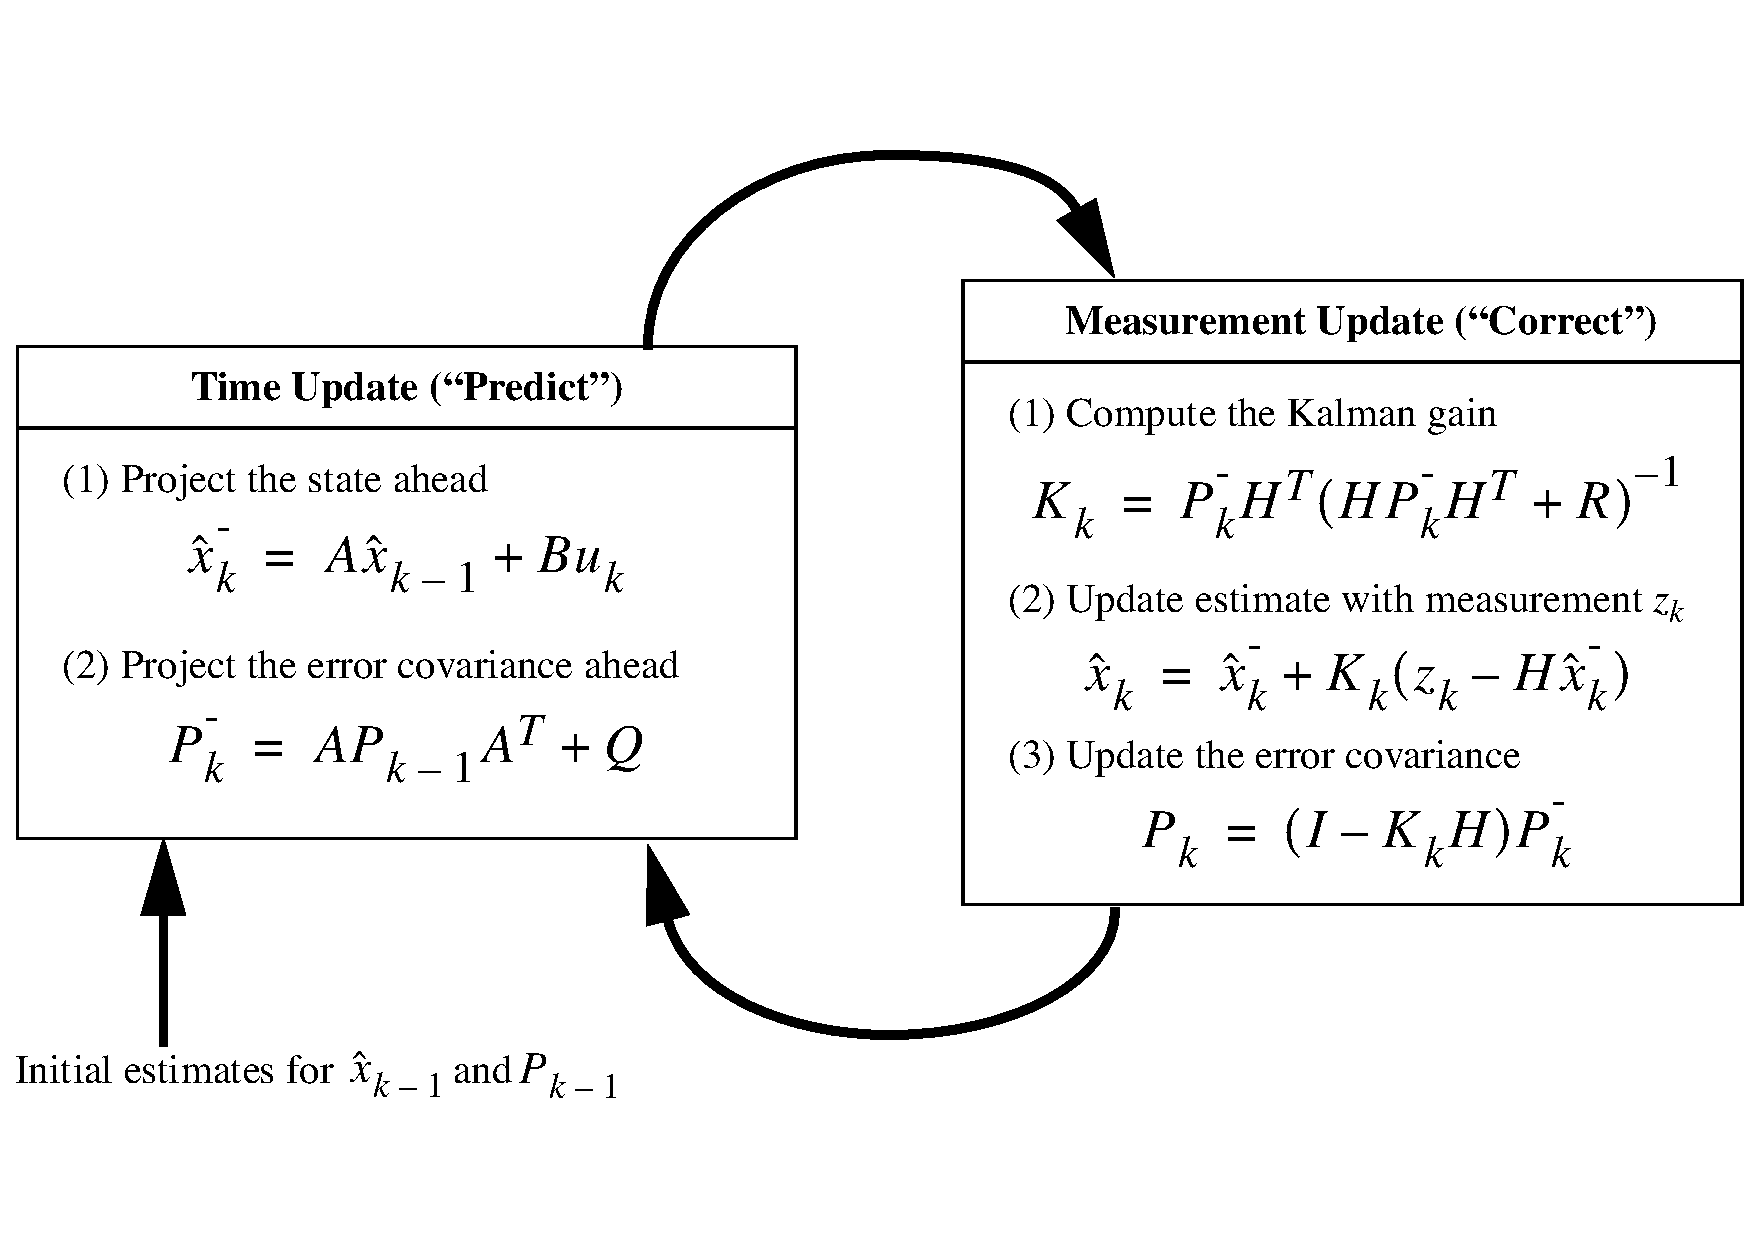
\includegraphics[trim=0cm 2cm 0cm 2cm, width=0.8\linewidth]{chapter_3_theoretical_background/KF_cycle.pdf}
	\caption[Overview of the \ac{KF} Predict-Update cycle]{Overview of the \ac{KF} Predict-Update cycle. The \ac{KF} keeps track of the estimated state of the system and the variance or uncertainty of the estimate. The estimate is updated using a state transition model and measurements.}
	Source: \textit{An introduction to the kalman filter} \cite{bishop2001introduction}
	\label{fig:chapter_3_theoretical_background/KF_cycle}
\end{figure}

The state estimation process is performed in two steps: the prediction step and the update step. In the prediction step, the current state of the system is predicted based on the previous state and a mathematical model of the system. In the update step, the predicted state is corrected based on a measurement from the sensors.

The prediction step can be represented using the following equations:

\begin{equation}
	\begin{split}
		\hat{x}_k^- = A \hat{x}_{k-1} + B u_k \\
		P_k^- = A P_{k-1} A^T + Q
	\end{split}
\end{equation}

where $\hat{x}_k^-$ is the predicted state of the system at time $k$, $\hat{x}_{k-1}$ is the estimated state of the system at time $k-1$, $A$ is the state transition matrix, $B$ is the control-input matrix, $u_k$ is the control input at time $k$, $P_k^-$ is the predicted error covariance matrix, and $Q$ is the process noise covariance matrix. Note that the state transition, control-input and process noise covariance matrix values do not depend on the time-step time $k$.

On the other hand, the update step can be represented using the following equations:

\begin{equation}
	\begin{split}
		K_k = P_k^- H_k^T (H P_k^- H^T + R)^{-1} \\
		\hat{x}_k = \hat{x}_k^- + K_k (z_k - H_k \hat{x}_k^-) \\
		P_k = (I - K_k H) P_k^-
	\end{split}
\end{equation}

where $K_k$ is the \ac{KF} gain, $H$ is the measurement matrix, $R_k$ is the measurement noise covariance matrix and $I$ the identity matrix of the corresponding dimension. The \ac{KF} gain determines the relative weight given to the predicted state and the measurement, and is adjusted based on the measurement noise covariance matrix. The measurement matrix relates the measurements to the state variables, and is used to convert the measurements into the same units as the state variables.

\subsection{Hungarian algorithm formulation}
\label{subsec:3_HA_formulation}

The \acf{HA} \cite{kuhn1955hungarian}, also known as the Kuhn-Munkres algorithm, is an efficient algorithm for solving the assignment problem in combinatorial optimization. An example to illustrate the \ac{HA} solution for an assignment problem involves finding the optimal assignment of $n$ workers to $n$ jobs, given the cost of assigning each worker to each job.

The \ac{HA} works by iteratively finding a set of independent zero-cost assignments, which correspond to a perfect matching in a bipartite graph. These assignments are then used to reduce the problem size and find a new set of independent zero-cost assignments, until all workers are assigned to jobs.

This algorithm has a time complexity of O($n^3$), which makes it one of the most efficient algorithms for solving the assignment problem. In this algorithm, the cost matrix C is assumed to be an $n \times n$ matrix, where each element $C_{i,j}$ represents the cost of assigning worker i to job j. The matrix M represents the matching, where each element $M_{i,j}$ is 1 if worker i is assigned to job j, and 0 otherwise.

\begin{algorithm}[]
	\SetAlgoLined
	\DontPrintSemicolon
	\SetKwInOut{Input}{Input}
	\SetKwInOut{Output}{Output}
	\Input{A cost matrix $C$ of size $n\times n$}
	\Output{A minimum cost perfect matching}
	Initialize the label vectors $u_i = \min_{j\in{1,\dots,n}} C_{i,j}$ and $v_j=0$ for all $i,j$;
	Initialize the empty matching $M$;
	\While{$|M| < n$}{
		Choose an unmatched row $i$;
		Initialize the set $T = {i}$ and the predecessor vector $P = \emptyset$;
		\While{true}{
			Let $S$ be the set of columns $j$ such that $i\in T$ and $C_{i,j} = u_i + v_j$;
			If $|S| > 0$, choose any column $j$ in $S$;
			\Else{
				Choose a column $j$ such that $v_j = \min_{k\in{1,\dots,n}} v_k$ and let $S$ be the set of rows $i$ such that $j\in M$ or $C_{i,j} = u_i + v_j$;
				Increment each $u_i$ for $i\in T$ by $\delta = \min_{i\in T,j\in S} (u_i+v_j-C_{i,j})$;
				Decrement each $v_j$ for $j\in S$ by $\delta$;
				\For{each row $i\in T$ and each column $j\in S$}{
					\If{$C_{i,j} = u_i+v_j$}{
						Add the edge $(i,j)$ to the alternating tree represented by $M$ and $P$;
						\If{$j$ is unmatched}{
							Augment $M$ along the alternating tree to create a larger matching;
							\Return the updated matching $M$;
						}
						\Else{
							Add $j$ to $T$ and continue the while loop;
						}
					}
				}
			}
		}
	}
	\caption{The Hungarian algorithm for solving the minimum cost perfect matching problem}
	\label{alg:3_ha}
\end{algorithm}

As observed in Algorithm \ref{alg:3_ha}, the \ac{HA} iteratively finds an uncovered zero in the cost matrix C and adds it to the matching M, while also adjusting the cost matrix to ensure that all rows and columns are covered by the matching. This is done by finding the minimum uncovered cost in each row and subtracting it from all uncovered costs in the row, and finding the minimum cost in each uncovered column and adding it to all uncovered costs in the column. Once all rows and columns are covered, the algorithm returns the final matching $M$.

In conclusion, the \ac{HA} is a powerful optimization algorithm that solves the assignment problem in polynomial time. The algorithm has a wide range of applications and can be easily adapted to handle various constraints and objectives. The algorithm is also guaranteed to find the optimal solution to the assignment problem, which makes it a valuable tool in many practical settings.
	
\subsection{State Transition Equations of Single-Trajectory Models}
\label{subsec:3_state_transitions_single_traj}

As illustrated in Chapter \ref{cha:related_works}, Single-Trajectory prediction methods are used in the field of motion estimation and control, to predict the future state of an object based on its current state and motion. In these methods, the agents are mostly assumed to comply with motion models that describe their dynamic behavior in such a way these are not able to consider the road-related factors and the uncertainty of the current state is unreliable for long-term prediction. Then, these models should only be used for estimating uni-modal trajectories of the surrounding agents in the short-term (no more than 1-s).

\begin{figure}[h]
	\centering
	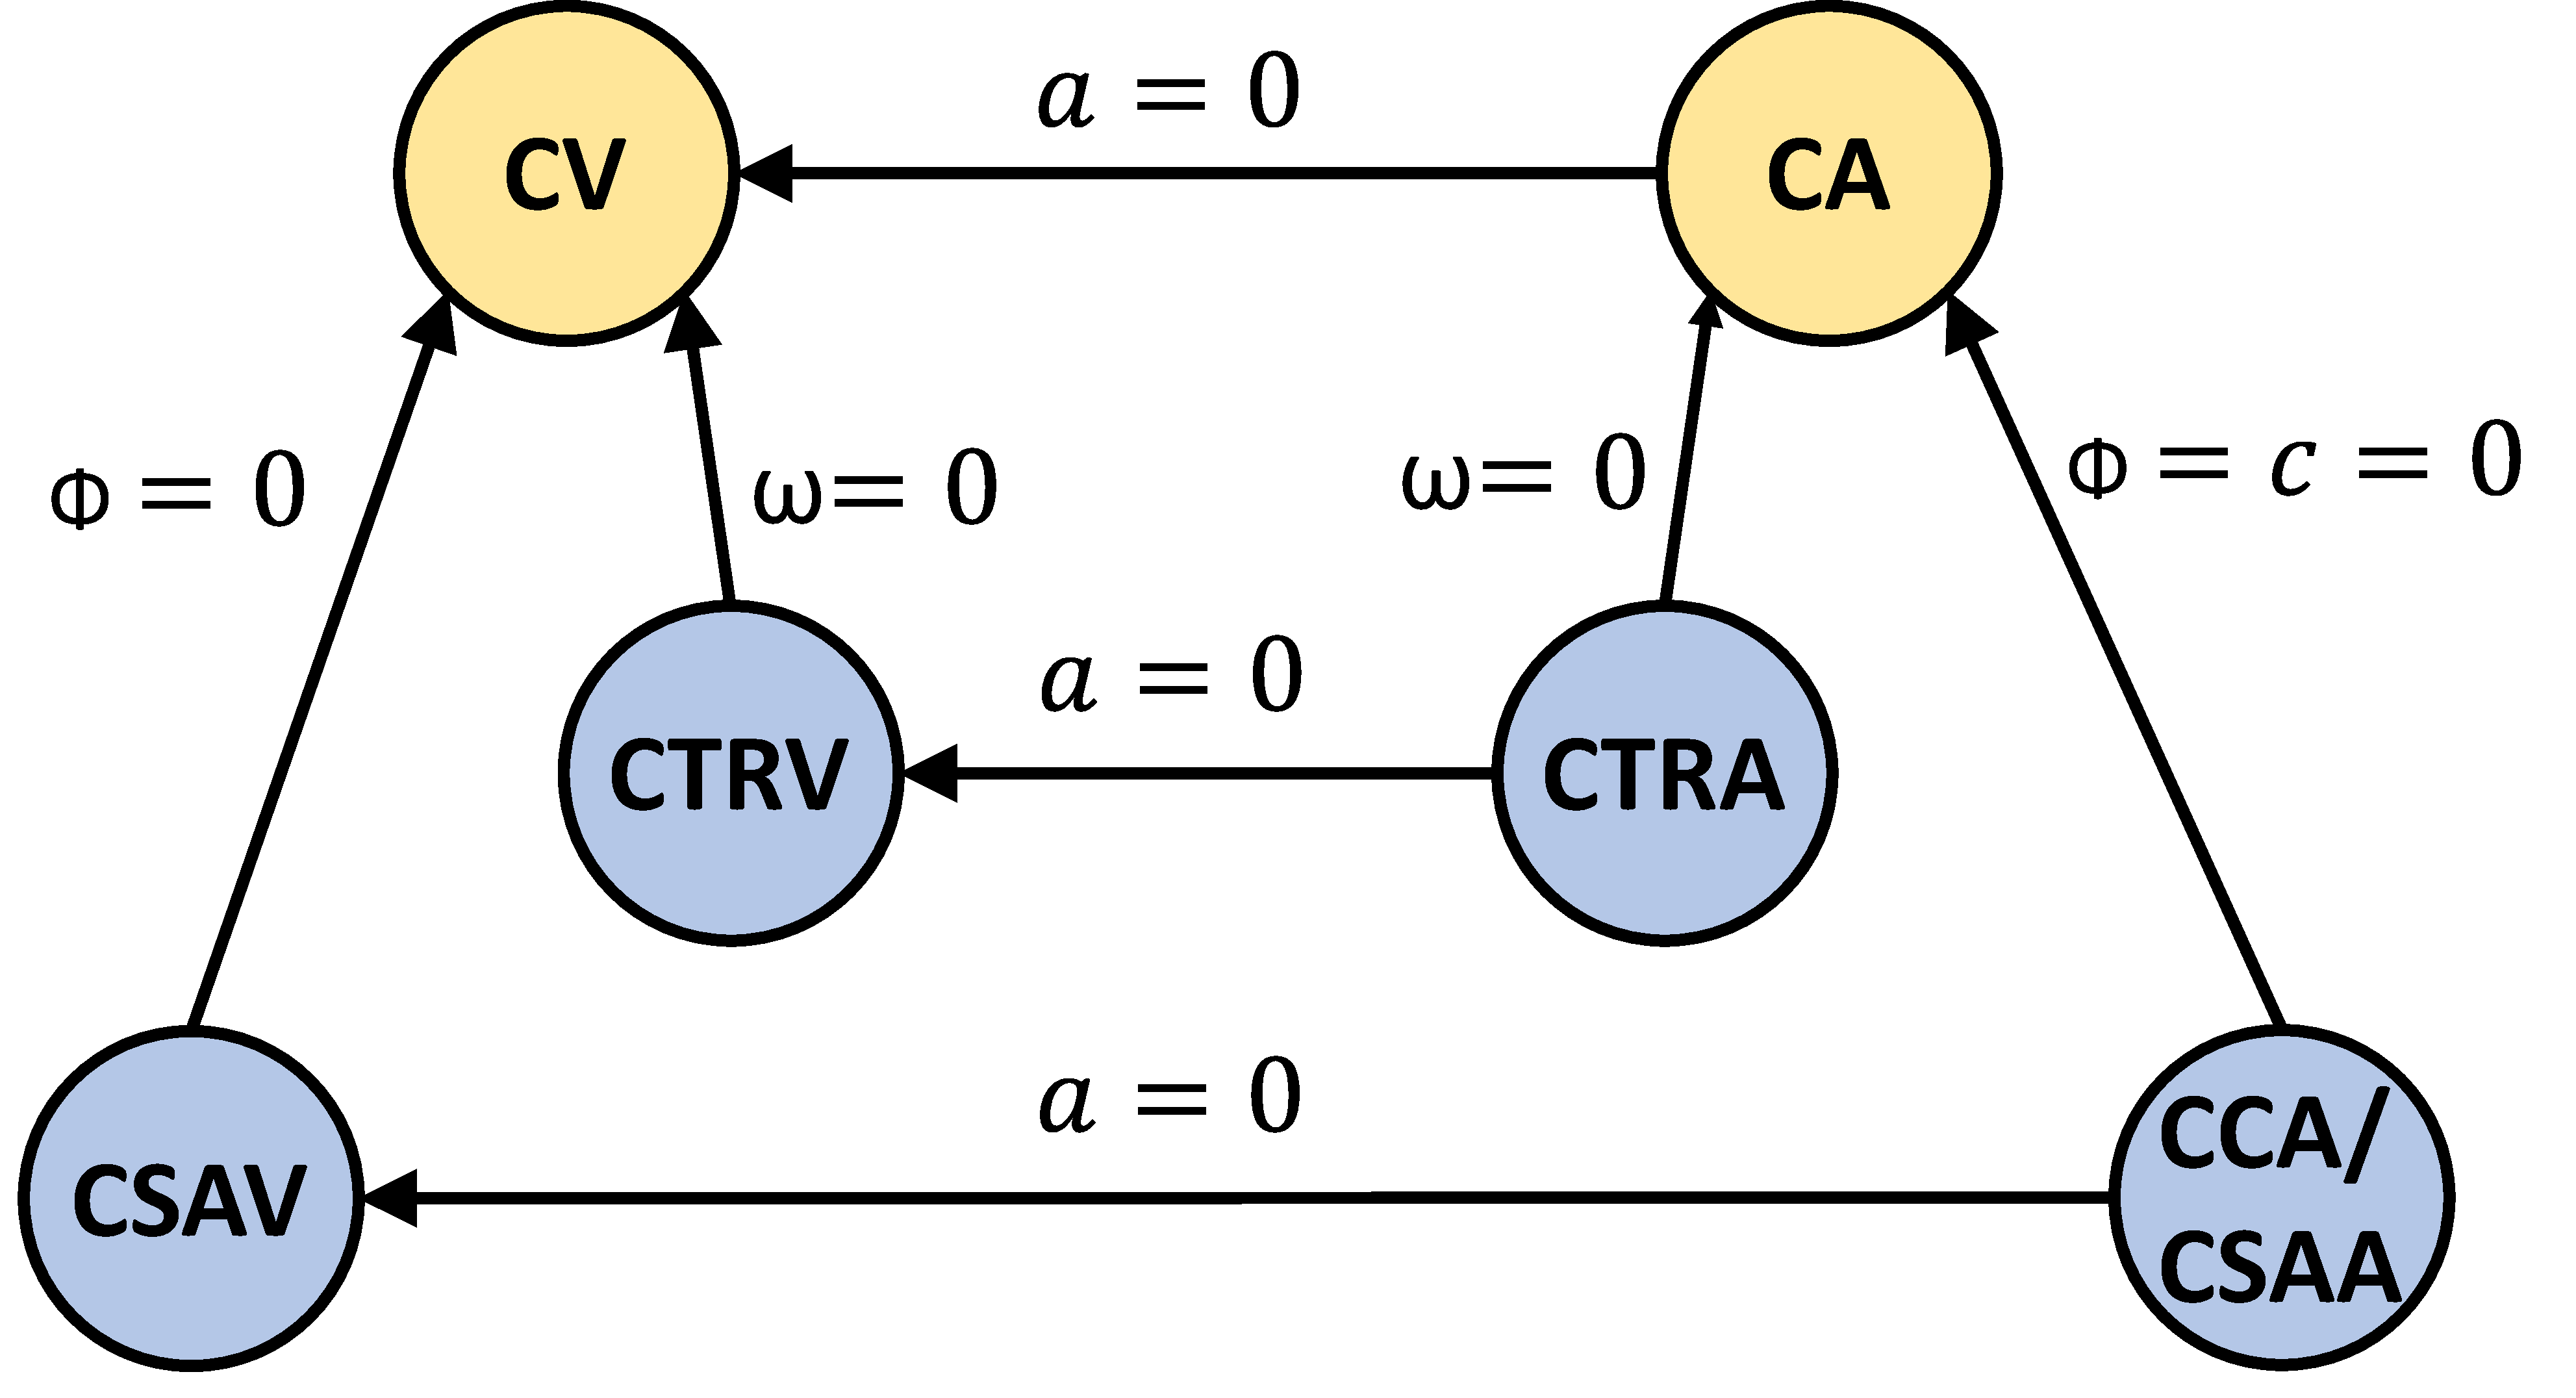
\includegraphics[width=0.6\linewidth]{chapter_3_theoretical_background/linear_curvilinear_mp.pdf}
	\captionsetup{justification=justified}
	\caption[Overview of Single Trajectory prediction methods]{Overview of Single Trajectory prediction methods. Every sophisticated model can be transformed into a simpler one by setting one state veriable to zero. $a$, $\phi$, $c$, $\omega$ represent the agent acceleration, steering angle, curvature and yaw rate (angular velocity) respectively}
	Source: \textit{Comparison and evaluation of advanced motion models for vehicle tracking} \cite{schubert2008comparison}
	\label{fig:chapter_3_theoretical_background/linear_curvilinear_mp}
\end{figure}

% including Constant Velocity (CV), Constant Acceleration (CA), Constant Turn Rate and Velocity (CTRV), Constant Turn Rate and Acceleration (CTRA), Constant Speed and Angular Velocity (CSAV), and Constant Curvature Acceleration (CCA)/Constant Speed and Angular Acceleration (CSAA)

Several single-trajectory prediction models have been proposed in the literature, as illustrated in Figure \ref{fig:chapter_3_theoretical_background/linear_curvilinear_mp}:

\begin{itemize}
	
	\item \acf{CV} model assumes that the object moves at a constant velocity and its future position can be predicted by simply extrapolating its current velocity vector. This model is simple and computationally efficient, but it may not accurately capture the object motion if it changes its velocity.
	
	\item \acf{CA} model is an extension of the CV model, assuming that the object can also change its acceleration in a linear manner. This model can provide more accurate predictions of the object future position and velocity, but it may not be suitable for objects with more complex motion patterns.
	
	\item \acf{CTRV} model assumes that the object moves in a circular trajectory with a constant turn rate and velocity magnitude. This model is useful for predicting the motion of objects such as drones or missiles, but it may not accurately represent the motion of objects with more complex trajectories.
	
	\item \acf{CTRA} model is an extension of the \ac{CTRV} model, allowing the object to change its acceleration while maintaining a constant turn rate. This model is often used in applications such as autonomous driving or aircraft navigation, where objects can accelerate or decelerate.
	
	\item \acf{CSAV} model assumes that the object moves along a straight line with a constant speed and acceleration vector. This model can be useful for predicting the motion of objects such as trains or boats. 
	
	\item \acf{CCA} model assumes that the object moves along a constant heading angle and can change its acceleration in a linear manner, also referred in the literature as \acf{CSAA} if the steering angle is used as a state variable instead of the curvature. From an algorithmic point of view, however, both names refer to the same model, which can be useful for predicting the motion of objects such as bicycles or motorcycles.
	
\end{itemize}

It can be observed how a sophisticated model can be transformed into a simpler one by setting one state variable to zero. For example, \ac{CTRA} is transformed to \ac{CTRV} if the agent acceleration $a$ is set to zero. Similarly, \ac{CTRA} is transformed to CA if the angular velocity $\omega$ is set to 0. In this Section we particularly focus on the prediction equations and differences of the most commonly used single-trajectory prediction methods in the field of \ac{AD}: \ac{CTRV} and \ac{CTRA}.

\subsubsection{Constant Turn Rate Velocity (CTRV)}
\label{subsubsec:3_CTRV}

The \acf{CTRV} model is a mathematical model used in the field of autonomous navigation to predict the future motion of a moving object. The model assumes that the agent moves along a smooth, continuous path, \ie \ the velocity and turn rate remain constant throughout the prediction interval.

With this model we are able to describe and predict the motion of the object using a set of differential equations that relate the rate of change of the agent state to its current state and any external inputs. It uses as main variables the current position, velocity, heading angle, and turn rate, and propagating them forward in time. % The state of the agent is described using five variables: the x and y coordinates of its position, its velocity magnitude, its heading angle (or direction of travel), and its turn rate.

The prediction equations for the CTRV model are described as follows:

\begin{equation}
\begin{split}
	x_{k+1} &= x_k + \frac{v_k}{\omega_k}\left[\sin(\psi_k+\omega_k\Delta t)-\sin(\psi_k)\right] \\
	y_{k+1} &= y_k + \frac{v_k}{\omega_k}\left[\cos(\psi_k)-\cos(\psi_k+\omega_k\Delta t)\right] \\
	v_{k+1} &= v_k \\
	\psi_{k+1} &= \psi_k + \omega_k\Delta t \\
	\omega_{k+1} &= \omega_k
\end{split}
\end{equation}
	
where $x_k$ and $y_k$ are the coordinates of the agent position, $v_k$ is the velocity magnitude, $\psi_k$ is the heading angle (in radians), $\omega_k$ is the turn rate (in radians per second) and $\Delta t$ is the time step size at timestep $k$ respectively.

The first two equations predict the agent position at the next time step, based on its current position, velocity, heading angle, and turn rate. The third and fifth equations predict that the velocity and turn rate will remain constant. The fourth equation predicts the object heading angle at the next time step, based on its current heading angle and turn rate.

\subsubsection{Constant Turn Rate Acceleration (CTRA)}
\label{subsubsec:3_CTRA}

The \acf{CTRA} model is an extension of the Constant Turn Rate and Velocity (CTRV) model, allowing the agent to change its acceleration while maintaining a constant turn rate. % This makes the \ac{CTRA} model more accurate for predicting the motion of objects that can accelerate or decelerate, such as cars or aircraft.

% The state of the agent in the CTRA model is described using variables such as the x and y coordinates of its position, its velocity magnitude, its heading angle, its turn rate, and its acceleration magnitude. 

The motion of the \ac{CTRA} agent is modeled using the following set of equations:

\begin{equation}
\begin{split}
		x_{k+1} &= x_k + \frac{v_k}{\omega_k} \left[ \sin(\theta_k + \omega_k \Delta t) - \sin(\theta_k) \right] \\
		y_{k+1} &= y_k - \frac{v_k}{\omega_k} \left[ \cos(\theta_k + \omega_k \Delta t) - \cos(\theta_k) \right] \\
		\theta_{k+1} &= \theta_k + \omega_k \Delta t \\
		v_{k+1} &= v_k + a_k \Delta t \\
		\omega_{k+1} &= \omega_k
\end{split}
\end{equation}

where the variables are the same than the \ac{CTRV} but at this point including the heading angle $\theta_k$ and agent acceleration $a_k$ at timestep $k$.

The first two equations describe the agent position updates based on its current position, velocity, heading angle, turn rate, and the time step. The third equation describes the agent heading angle update based on its current heading angle and turn rate. The fourth equation describes the agent velocity update based on its current velocity and acceleration. The last equation assumes that the agent turn rate remains constant over time.

As observed, the prediction equations for the \ac{CTRV} model are based on the kinematic equations for circular motion, where the object position, velocity, and heading angle change in a continuous and smooth manner. In contrast, the prediction equations for the \ac{CTRA} model include an additional term for the object acceleration, which allows for more accurate predictions of the object future motion when it can accelerate or decelerate.

In terms of implementation, the \ac{CTRA} model requires more computational resources due to the additional term for acceleration, which increases the complexity of the equations. This can make the \ac{CTRV} model more computationally efficient and faster to calculate in real-time applications. 

\section{Deep Learning algorithms}
\label{sec:3_dlb_formulation}

In this section the mathematical formulation of the \ac{DL} layers employed in this thesis is covered. In particular, these are the 1D-\ac{CNN}, \ac{LSTM}, \ac{cGAN}, Attention mechanism and \ac{GCN} layers. We briefly introduce each layer, as well as the corresponding mathematical formulation to enhance the comprehension of the learning-based methods proposed in future Chapters.

\subsection{Convolutional Neural Networks (CNNs)}
\label{subsec:3_cnns}

% Additional info

% https://towardsdatascience.com/understanding-1d-and-3d-convolution-neural-network-keras-9d8f76e29610
% file:///C:/Users/Carlos/Downloads/sensors-22-09517.pdf
% https://e2eml.school/convolution_one_d.html
% https://arxiv.org/pdf/1512.07108.pdf

\acp{CNN} are commonly used for image and signal processing tasks. The type of \ac{CNN} architecture used depends on the nature of the input data. Here are the differences among the three main types of \acp{CNN}:

\begin{itemize}
	
	\item \textbf{1D Convolutional Neural Networks (1D-\acp{CNN})} are used for processing sequential data such as time series data, speech signals or text data. The input is a one-dimensional sequence of data, such as a time series of sensor readings. 1D-\acp{CNN} typically have fewer parameters and are computationally efficient compared to 2D- and 3D-\acp{CNN}.
	
	\item \textbf{2D Convolutional Neural Networks (2D-\acp{CNN})} are used for processing 2D images. The input is a two-dimensional image represented as a matrix of pixels. The convolutional layers in a 2D-\ac{CNN} apply filters that slide over the image to extract local features. The output of each convolutional layer is a set of 2D feature maps. 2D-\acp{CNN} are widely used for image classification, object detection, and image segmentation.
	
	\item \textbf{3D Convolutional Neural Networks (3D-\acp{CNN})} are used for processing 3D volumetric data such as CT scans, MRI images, and video data. The input is a three-dimensional volume represented as a sequence of 2D images. The convolutional layers in a 3D-\ac{CNN} apply filters that slide over the 3D volume to extract local features. The output of each convolutional layer is a set of 3D feature maps. 3D-\acp{CNN} are used for tasks such as medical image analysis, video classification, 3D object detection and action recognition.
	
\end{itemize}

As we will see in further Chapters, in this work we focus on 1D-\acp{CNN}. The basic building blocks of a 1D \ac{CNN} are convolutional layers, which learn local patterns in the input data by applying a set of filters to it, as illustrated in Figure \ref{fig:chapter_3_theoretical_background/CNN_1D}. Each filter slides over the input sequence and performs a dot product operation at each position to generate a feature map. These feature maps capture the presence of certain patterns at different positions in the input sequence. 
 
The architecture of a 1D-\ac{CNN} typically consists of several convolutional layers, followed by one or more fully connected layers for classification or regression. The output of each convolutional layer is fed into the next layer, with optional pooling layers in between to reduce the spatial dimension of the feature maps, which are finally flattened before the final layer. The output of the network is obtained by passing the output of the last fully connected layer through a suitable activation function, such as softmax for classification or linear for regression.
 
 \begin{figure}[h]
 	\centering
 	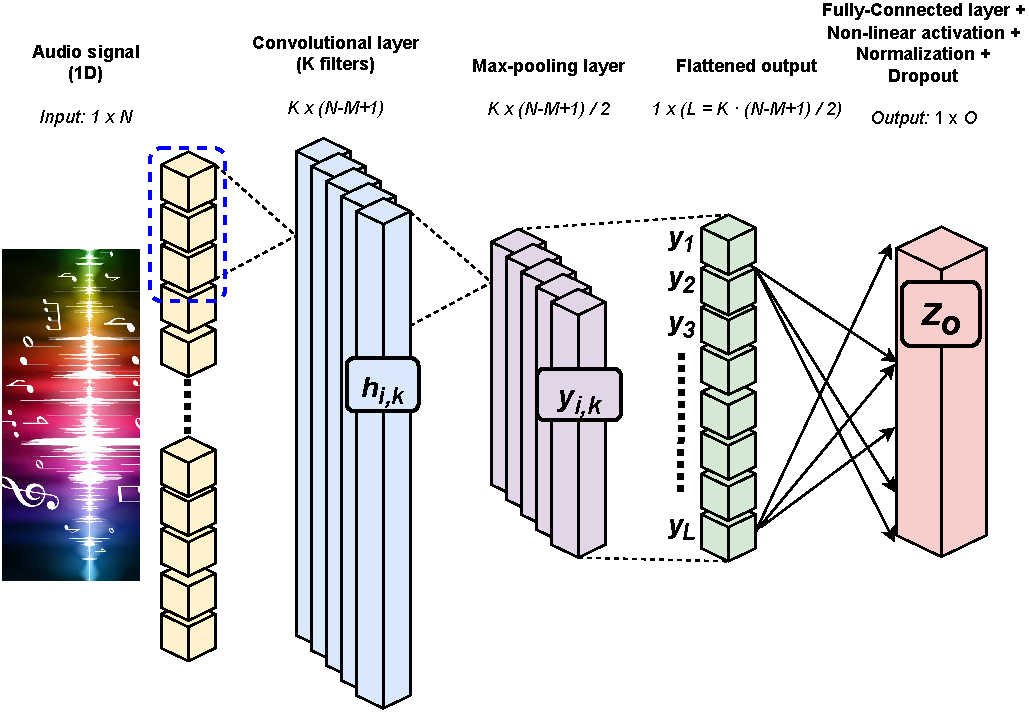
\includegraphics[width=0.6\linewidth]{chapter_3_theoretical_background/CNN_1D.pdf}
 	\caption{Example of a Convolutional Neural Network (CNN) architecture to process 1D-input signals}
 	\label{fig:chapter_3_theoretical_background/CNN_1D}
 \end{figure}
 
Let $x$ be a 1-dimensional input sequence of length $N$, represented as a vector $x = [x_1, x_2, ..., x_N]$. Let $K$ be a set of filters of length $M$, represented as a vector $k = [k_1, k_2, ..., k_M]$. We can apply the filter $k$ to the input sequence $x$ by computing a convolution operation:

\begin{equation}
	(k * x)_i = \sum_{j=1}^M k_j x_{i+j-M}
\end{equation}

where $*$ denotes the convolution operation, and $i$ ranges from $M$ to $N$. This operation produces a new sequence of length $N - M + 1$, representing the local features extracted from the input sequence $x$ by the filter $k$. 

To extract different types of features, we apply $K$ filters in each convolutional layers in the network. Then, each layer applies a set of filters, and produces a set of feature maps. The feature maps can be computed as:

\begin{equation}
	h_{i,k} = f(\sum_{k=1}^M W_{j,k} x_{i+k-M} + b_j)
\end{equation}

where $h$ is the feature map at position $i$ and filter $k$, $W$ is the weight matrix of the $k$-th filter, $b$ is the bias term for the $k$-th filter, and $f$ is an activation function (such as ReLU or sigmoid). Note that in Figure \ref{fig:chapter_3_theoretical_background/CNN_1D} a bench of $K=4$ filters is applied in the convolutional layer.

After each convolutional layer, we typically apply a pooling layer to reduce the dimensionality of the features and increase the translation invariance of the network. The most common pooling operation is max pooling, which selects the maximum value within a window of size $p$:

\begin{equation}
	y_{i,k} = \max_{j=0}^{p-1} h_{i+k,j}
\end{equation}

where $y$ is the output of the pooling layer at position $i$ and filter $k$. After this operation, feature dimensionality is normally halved ($L = (N-M+1) / 2$), as observed in Figure \ref{fig:chapter_3_theoretical_background/CNN_1D}. Once we have the corresponding features maps after the max pooling operation, we typically take the output of the pooling layer and flatten into a vector of $L$, and fed into a set of fully connected layers, with optional dropout regularization and batch normalization

Finally, we can use one or more fully connected layers to perform the final classification or regression task. The output of the pooling layer is flattened into a vector of length $O$, and fed into a set of fully connected layers, with optional dropout regularization and batch normalization:

\begin{equation}
	z_o = f(\sum_{o=1}^O W_{l,o} y_l + b_o)
\end{equation}

where $z_{o}$ is the o-th element of the output vector with length O, $W$ is the weight matrix, $y$ is the flattened output of the pooling layer with length $L$, $b$ is the bias term, and $f$ is an activation function. 

We make use of the 1D-\ac{CNN} mechanism in Chapters \ref{cha:efficient_baseline_for_mp_in_ad} and \ref{cha:improving_multi_agent}, studying its effect in our algorithms, leveraging its wider receptive field compared with a \ac{MLP} to reduce the influence of noisy input data. 

\subsection{Recurrent Neural Networks (RNNs)}
\label{subsec:3_rnns}

\acfp{RNN} are a type of neural network that are designed to process sequential data, where the order of the input matters, usually assuming the presence of discrete timestep. They are widely used in a variety of applications such as natural language processing, speech recognition, image captioning, and time series prediction.

The general theory of \acp{RNN} is that they have a feedback loop in their architecture that allows information to be passed from one time step to the next, thereby enabling the network to capture dependencies between the inputs at different time steps. The input at each time step is fed into the network along with the output from the previous time step, and the network uses this information to generate a new output.

There are several types of \acp{RNN}, including the basic \ac{RNN}, the \ac{GRU}, and the \acf{LSTM} \cite{hochreiter1997long}. The basic \ac{RNN} is the simplest form of \ac{RNN}, where the output at each time step is a function of the input at that time step and the output from the previous time step. However, it suffers from the vanishing gradient problem, where the gradients become exponentially small as they propagate through time, making it difficult to learn long-term dependencies.

The \ac{GRU} is a variation of the basic \ac{RNN} that uses gating mechanisms to control the flow of information through the network. It has fewer parameters than the \ac{LSTM} and can be faster to train, but it may not perform as well as the \ac{LSTM} on tasks that require more complex temporal dependencies.

\subsubsection{Long Short-Term Memory (LSTM)}
\label{subsubsec:3_LSTMs}

\ac{LSTM} networks were introduced to address the vanishing gradient problem in standard \acp{RNN}. They achieve this by using a memory cell to store information over long periods of time, and three gating mechanisms to control the flow of information through the network. Figure \ref{fig:chapter_3_theoretical_background/LSTM} provides a detailed overview of the \ac{LSTM} cell structure, illustrating the workflow from the previous cell output and input at time $t-1$ in order to compute the current cell state and hidden state at time $t$.

\begin{figure}[h]
	\centering
	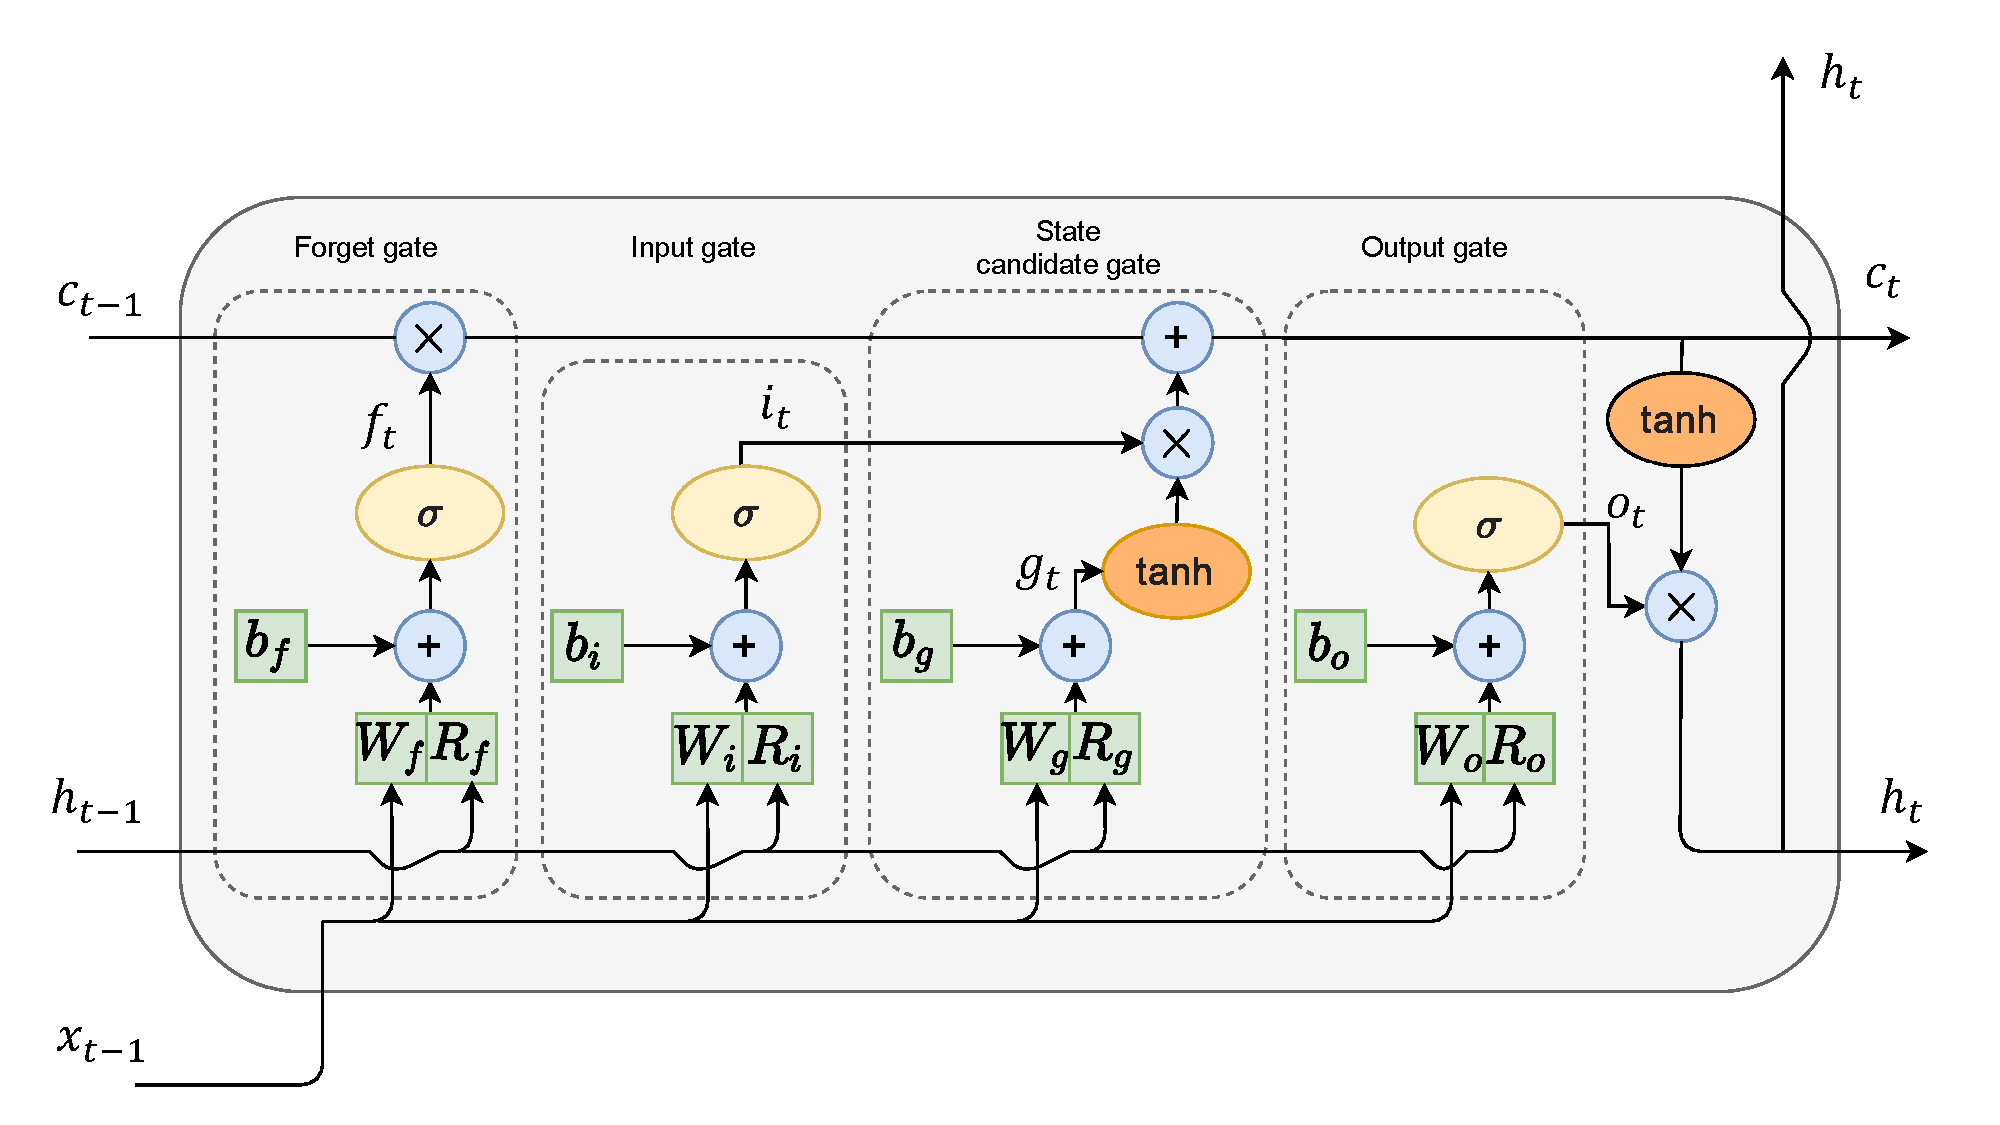
\includegraphics[width=\linewidth]{chapter_3_theoretical_background/LSTM_cell.pdf}
	\caption{Overview of the LSTM cell structure}
	\label{fig:chapter_3_theoretical_background/LSTM}
\end{figure}

The three gates are called the input gate, forget gate, and output gate, and they are responsible for deciding which information to store in the memory cell, which information to forget, and which information to output, respectively.

The equations for the input, forget, and output gates are as follows:

\begin{itemize}
	\item \textbf{Input gate}: $i_k = \sigma(W_i R_i \cdot [h_{k-1}, x_k] + b_i)$
	\item \textbf{Forget gate}: $f_k = \sigma(W_f R_f * [h_{k-1}, x_k] + b_f)$
	\item \textbf{Output gate}: $o_k = \sigma(W_o R_o * [h_{k-1}, x_k] + b_o)$
\end{itemize}

where $x_k$ is the input at the current timestep $k$, $h_{k-1}$ is the hidden state from the previous timestep, $i_k$ is the input gate activation, $f_k$ is the forget gate activation, and $o_k$ is the output gate activation for the current timestep $k$ respectively. On the other hand, $W_i R_i$, $W_f R_f$, and $W_o R_o$ are weight matrices (where the component W denotes the weights associated with the input signals $x$ and R denotes the so-called recursive weights, associated with the hidden state of the cell from the previous timestep), and $b_i$, $b_f$, and $b_o$ are bias vectors.

Moreover, the memory cell is updated based on the input, forget, and output gates, as well as a new candidate value that is computed based on the current input and hidden state. The equations for the memory cell and candidate value are as follows:

\begin{equation}
\begin{split}
		C_k &= f_k \cdot C_{k-1} + i_k \cdot \tilde{C}_k \\
		\tilde{C}_k &= \tanh(W_g R_g \cdot [h_{k-1}, x_k] + b_g)
\end{split}
\end{equation}

where $\tilde{C}_k$ is the candidate value, $C_t$ is the new memory cell value, and $C_{k-1}$ is the previous memory cell value. 

Finally, the hidden state at time $t$ is computed based on the output gate and the new memory cell value, using the following equation:

\begin{equation}
	h_k = o_k \cdot \tanh(C_k)
\end{equation}

This equation scales the memory cell value by the output gate activation, then applies a hyperbolic tangent function to obtain the new hidden state.

In summary, \acp{LSTM} use a memory cell and three gating mechanisms to learn long-term dependencies in sequential data. The input, forget, and output gates control the flow of information through the network, while the memory cell stores information over time. The equations for \acp{LSTM} involve computing the input, forget, and output gate activations, the candidate value, the new memory cell value, and the new hidden state.

We make use of the \ac{LSTM} network in Chapters \ref{cha:exploring_gan_for_vehicle_mp} and \ref{cha:efficient_baseline_for_mp_in_ad} due to its powerful ability to represent as a high-dimensional space the past/future trajectories of the agents, though, as it will be seen in Section \ref{subsec:3_attention} of this Chapter, for the final proposal of the thesis we employ transformer-based modules since they are more powerful than \ac{LSTM} and easier to train.

\subsection{Generative Adversarial Networks (GANs)}
\label{subsec:3_gans}

A discriminative model is a type of machine learning model that learns the relationship between the input features and the target output directly. The goal of a discriminative model is to learn a decision boundary that separates different classes in the input data. In other words, discriminative models focus on learning the conditional probability distribution of the target variable given the input features.

Discriminative models are often used in supervised learning tasks, such as classification and regression, where the goal is to predict a target variable based on a set of input features. Common examples of discriminative models include logistic regression, support vector machines, and neural networks.

Unlike generative models, which learn the joint probability distribution of the input and target variables, discriminative models do not model the probability distribution of the input data explicitly. Instead, they focus on learning a mapping function that directly maps the input features to the target output.

\begin{figure}[h]
	\centering
	\includegraphics[trim=0cm 8cm 0cm 0cm, width=\linewidth]{chapter_3_theoretical_background/GAN_diagram.pdf}
	\caption{Overview of a \ac{GAN} structure}
	\label{fig:chapter_3_theoretical_background/GAN}
\end{figure}

In 2014, a breakthrough paper introduced \acfp{GAN} \cite{goodfellow2020generative}, a clever new way to leverage the power of discriminative models to get good generative models. At their heart, \acp{GAN} rely on the idea that a data generator is good if we cannot tell fake data apart from real data. In statistics, this is called a two-sample test, a test to answer the question whether datasets $X=\{x_1,\ldots, x_n\}$ and $X'=\{x'_1,\ldots, x'_n\}$ were drawn from the same distribution. This allows to improve the data generator until it generates something that resembles the real data. At the very least, it needs to fool the classifier even if our classifier is a state of the art deep neural network. \acp{GAN} are a powerful technique for generating realistic samples that are similar to some training data. As observed in Figure \ref{fig:chapter_3_theoretical_background/GAN}, a \ac{GAN} consists of two neural networks, a generator network and a discriminator network. The generator and discriminator networks are trained in a two-player game, where the generator tries to produce samples that fool the discriminator, and the discriminator tries to correctly classify between real and generated data. The objective function for a \ac{GAN} is a min-max game between the generator and discriminator, and can be optimized using gradient descent or some other optimization algorithm. Some common applications where \acp{GAN} are widely used are generating realistic images, videos, audio, data augmentation or style transfer.

The generator network takes as input a random noise vector, and generates a sample that is meant to mimic real data. The discriminator network takes as input a sample, and tries to distinguish between real data and generated data. The two networks are trained in a two-player game, where the generator tries to produce samples that fool the discriminator, and the discriminator tries to correctly classify between real and generated data.

The objective function for a \ac{GAN} can be formulated as a min-max game between the generator and discriminator. The generator tries to minimize the probability that the discriminator correctly classifies the generated samples as fake, while the discriminator tries to maximize the probability that it correctly classifies the real and generated samples.

The objective function for a \ac{GAN} can be written as:

\begin{equation}
\begin{split}
	\min_{\theta_G}\max_{\theta_D} V(D, G) = \mathbb{E}_{x\sim p_{data}(x)}[\log D(x)] + \mathbb{E}_{z\sim p_z(z)}[\log(1-D(G(z)))] \\
	= \mathbb{E}_{x\sim p_{data}(x)}[\log D(x)] + \mathbb{E}_{z\sim p_z(z)}[\log(1-D(G(z;\theta_G)))]
\end{split}
\end{equation}

where $\theta_G$ and $\theta_D$ are the parameters of the generator and discriminator networks, respectively, $x$ is a real sample from the training data distribution $p_{data}$, $z$ is a noise vector sampled from a prior distribution $p_z$, and $G(z;\theta_G)$ is the generated sample from the generator network.

The first term of the objective function represents the expected log-probability of the discriminator correctly classifying a real sample as real. The second term represents the expected log-probability of the discriminator correctly classifying a generated sample as fake.

During training, the generator network is updated to minimize the objective function with respect to $\theta_G$, while the discriminator network is updated to maximize the objective function with respect to $\theta_D$. This can be done using gradient descent or some other optimization algorithm.

There are some well-known types of \acp{GAN}, such as:

\begin{itemize}
	\item \textbf{Deep Convolutional GANs (DCGANs)}: These are \acp{GAN} that use \acp{CNN} in the generator and discriminator networks. DCGANs are commonly used for image generation and have been shown to produce high-quality, realistic images.
	\item \textbf{Wasserstein GANs (WGANs)}: These are \acp{GAN} that use the Wasserstein distance instead of the traditional Kullback-Leibler (KL) divergence or Jensen-Shannon (JS) divergence for measuring the difference between the real and generated distributions. WGANs have been shown to produce more stable training and generate higher-quality samples.
	\item \textbf{CycleGANs}: These are \acp{GAN} that are designed for image-to-image translation tasks, where the goal is to transform an image from one domain to another. CycleGANs use two generators and two discriminators to learn the mapping between the two domains.
\end{itemize}

Nevertheless, in this work we focus on a particular type of \ac{GAN}, known as \acf{cGAN}, where the generator is conditioned on some additional information, allowing for more specific generation of data. 

\subsubsection{GAN vs cGAN}
\label{subsubsec:3_cGAN}

The main difference between the original \acf{GAN} and \acf{cGAN} is that the original \ac{GAN} generates samples without any control over the generated output, whereas the \ac{cGAN} generates samples conditioned on some additional information.

In the original \ac{GAN}, the generator network takes as input a random noise vector, and generates a sample that is meant to mimic real data. The discriminator network takes as input a sample, and tries to distinguish between real data and generated data. The goal of the original \ac{GAN} is to train the generator network to generate samples that are indistinguishable from real data.

\begin{figure}[h]
	\centering
	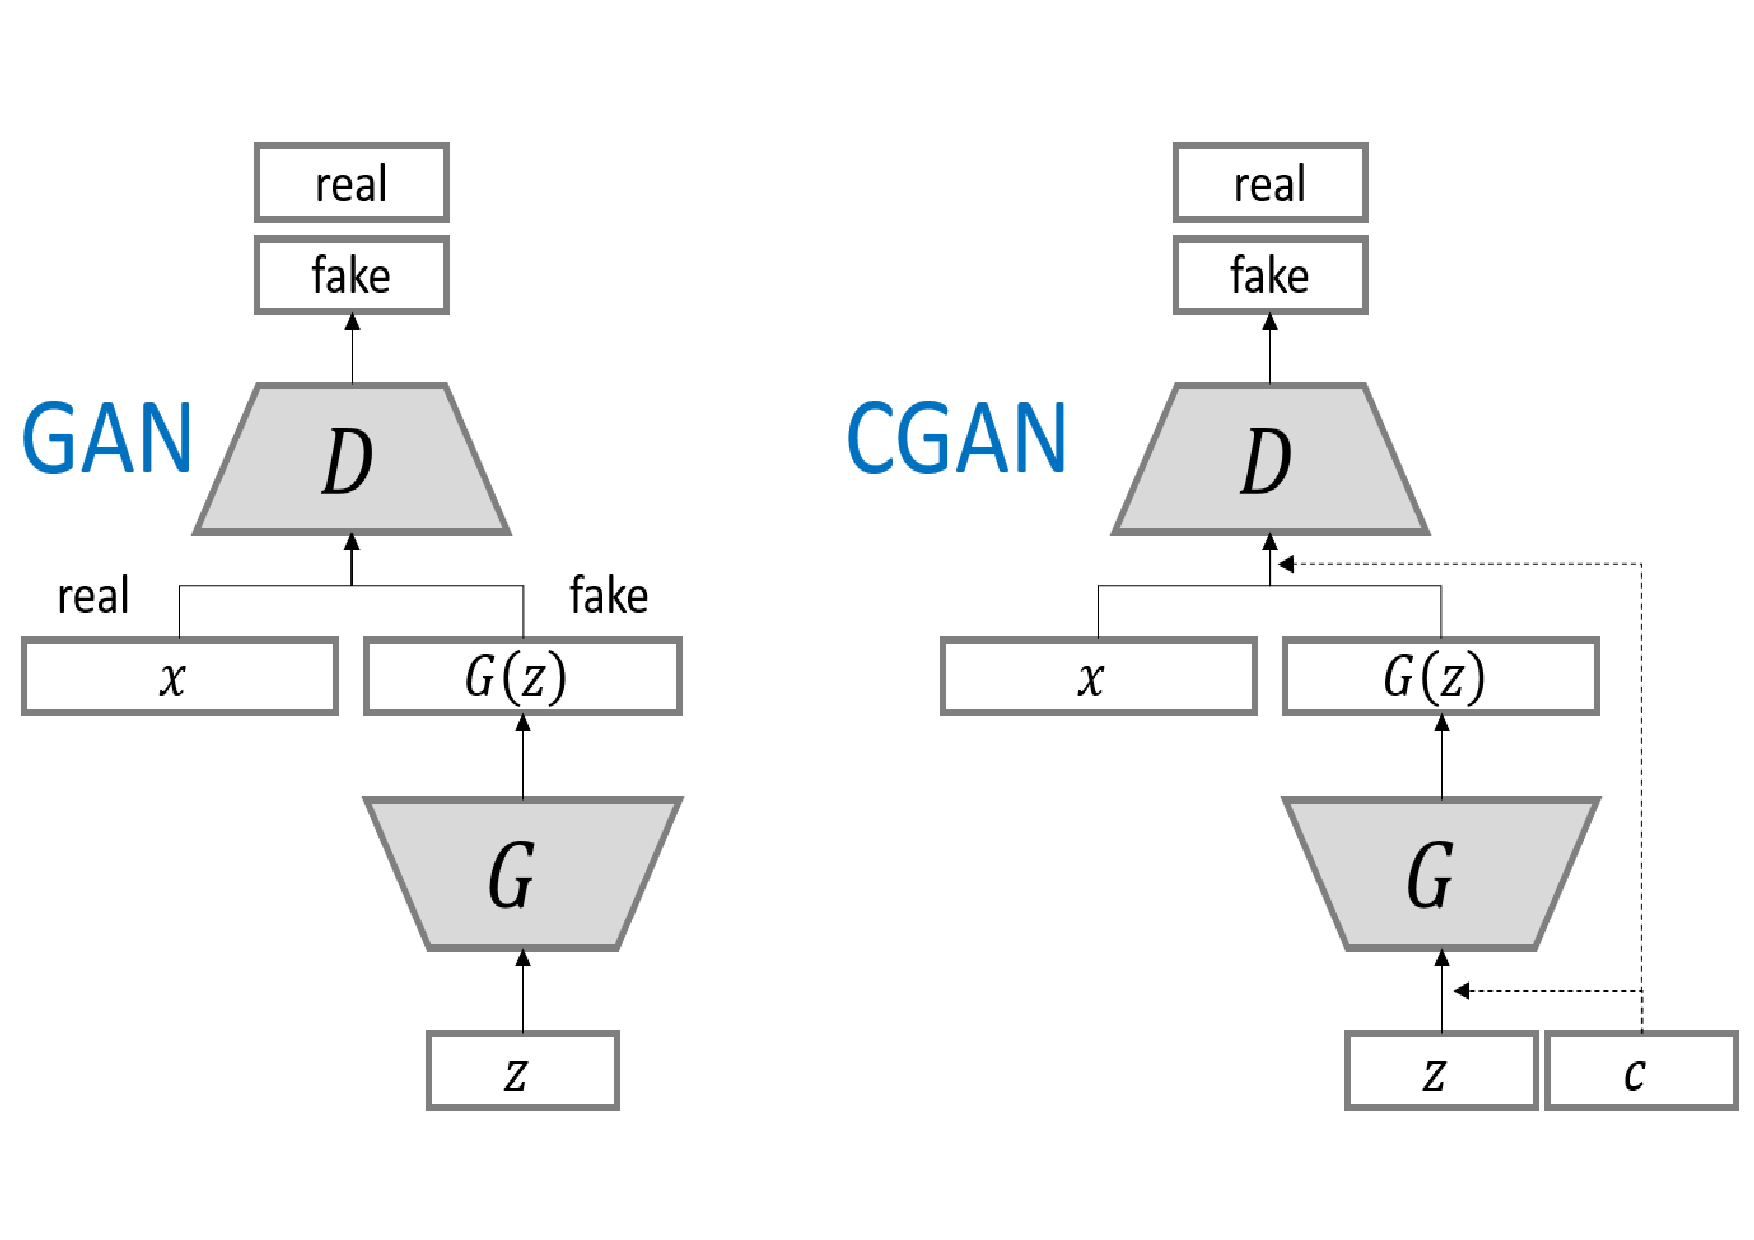
\includegraphics[trim=0cm 0.5cm 0cm 0.5cm, width=0.75\linewidth]{chapter_3_theoretical_background/GAN_vs_cGAN.pdf}
	\caption{Comparison between the original \ac{GAN} and \ac{cGAN}}
	Source: \textit{Logan: Generating logos with a generative adversarial neural network conditioned on color} \cite{mino2018logan}
	\label{fig:chapter_3_theoretical_background/GAN_vs_cGAN}
\end{figure}

In contrast, a \ac{cGAN} is a \ac{GAN} that is conditioned on some additional information, such as class labels or image annotations. The generator network in a \ac{cGAN} takes as input both a random noise vector and a condition vector, and generates a sample that is conditioned on the additional information. The discriminator network also takes as input both the sample and the condition vector, and tries to distinguish between real data and generated data based on the condition. Figure \ref{fig:chapter_3_theoretical_background/GAN_vs_cGAN} illustrates the differences between both architectures.

The \ac{cGAN} can be used for a variety of applications, such as image-to-image translation, where the additional information is an input image that is translated to a different output image. For example, a \ac{cGAN} can be trained to convert grayscale images to color images, or to transform images of one type of object to another type of object.

The training process for a \ac{GAN} is similar to that of the original \ac{GAN}, but the loss function for the generator and discriminator networks are modified to include the condition vector. Specifically, the loss function for the generator network includes a term that measures how well the generated samples match the condition vector, in addition to the term that measures how well the generated samples fool the discriminator. Similarly, the loss function for the discriminator network includes a term that measures how well the discriminator can identify the condition vector, in addition to the term that measures how well it can distinguish between real and generated data.

We make use a \ac{cGAN}-based approach in Chapter \ref{cha:exploring_gan_for_vehicle_mp} to compute plausible uni-modal predictions, where the input to the generative model (as we will see, represented by a \ac{LSTM} network) is a noise vector $z$ sampled from a multi-variate normal distribution and the physical and social represent the conditions to the model.

% The cGAN can be used for a variety of applications, such as image-to-image translation, where the additional information is an input image that is translated to a different output image. For example, a cGAN can be trained to convert grayscale images to color images, or to transform images of one type of object to another type of object.

\subsection{Attention Mechanism}
\label{subsec:3_attention}

The attention mechanism \cite{vaswani2017attention} is a computational method used in \ac{DL} models to help the model focus on the most important parts of the input data. It is commonly used in Natural Language Processing (NLP), speech recognition, and computer vision. In terms of \ac{MP}, the attention mechanism is usually employed to model interaction among entities (either social or physical) to compute the most important features once the corresponding encoders have previously computed a deep description of the scene, \ie \, attention is commonly employed to extract relevant information from high-dimensional vectors (\eg \ 64 or 128).

The basic idea of attention is to compute a set of weights that indicate the relative importance of different parts of the input. These weights are then used to compute a weighted sum of the input, which is used as the output of the attention mechanism. The attention mechanism can be formulated mathematically using the following equations:

\begin{itemize}
	\item First, we compute a set of \textit{keys}, \textit{values}, and a \textit{query} vector, which are used to compute the attention weights:
	
	\begin{equation}
		\begin{split}
			K = {k_1, k_2, ..., k_n} \\
			V = {v_1, v_2, ..., v_n} \\
			Q = {q_1, q_2, ..., q_d}
		\end{split}
	\end{equation}

	where $n$ is the number of elements in the input, and $d$ is the dimension of the query vector.
	
	\item Next, we compute the attention weights using a function that compares the query vector to each of the keys:
	
	\begin{equation}
		a_i = \text{softmax}(q^T k_i)
	\end{equation}
	
	where $a_i$ is the attention weight for the $i$-th element of the input. 
	
	\item Finally, we compute the output of the attention mechanism as a weighted sum of the values:
	
	\begin{equation}
		o = \sum_{i=1}^{n} a_i v_i
	\end{equation}
\end{itemize}

\subsubsection{Positional Encoding}
\label{subsubsec:3_positional_encoding}

In the attention mechanism, positional encoding is used to incorporate the order of the input sequence into the model. Positional encoding involves adding a fixed-length vector to the input embeddings that encodes the position of each element in the sequence. It has shown to be an effective way of incorporating sequential information into transformer-based in applications such  machine translation, language modeling, sentiment analysis or the present case, \ac{MP} in the field of \ac{AD}, where the order the sequence plays a fundamental role.

The mathematical formulation of positional encoding is as follows:

\begin{equation}
	\text{PE}_{(pos,2i)} = \sin\left(\frac{pos}{10000^{2i/d}}\right)
\end{equation}

\begin{equation}
	\text{PE}_{(pos,2i+1)} = \cos\left(\frac{pos}{10000^{2i/d}}\right)
\end{equation}

where $pos$ is the position of the element in the sequence, $i$ is the index of the dimension, and $d$ is the dimension of the input embeddings. The positional encoding vectors are added to the input embeddings before they are passed through the self-attention mechanism.

The choice of the hyperparameters used in the positional encoding formulation, such as the use of the sine and cosine functions and the value of $10000$, is arbitrary but has been shown to work well in practice. The positional encoding vectors add a sinusoidal pattern to the input embeddings that allows the model to distinguish between elements at different positions in the sequence.

\subsubsection{Multi-Head Attention}
\label{subsubsec:3_multi_head_attention}

Multi-head attention is a type of attention mechanism used in \ac{DL} models, particularly in transformer-based architectures. This Multi-Head concept allows the model where it is integrated to attend to multiple parts of the input at once, which is really useful for capturing complex relationships between different parts of the input. It involves splitting the input into multiple heads and computing separate attention scores for each head, which are then combined to produce the final output. It can be formulated mathematically using the following equations:

\begin{itemize}
	\item First, we split the keys, values, and query vectors into multiple \textit{heads}, each of which has its own set of learned weight matrices:
	
	\begin{equation}
		\begin{split}
			K_i = {k_{i,1}, k_{i,2}, ..., k_{i,n}} \\
			V_i = {v_{i,1}, v_{i,2}, ..., v_{i,n}} \\
			Q_i = {q_{i,1}, q_{i,2}, ..., q_{i,d}}
		\end{split}
	\end{equation}
	
	where $i$ is the index of the head. 
	
	\item Next, we compute the attention weights and outputs for each head separately, using the same equations as in the basic attention mechanism:
	
	\begin{equation}
		a_{i,j} = \text{softmax}(Q_i^T K_{i,j})
	\end{equation}
	
	\begin{equation}
		o_{i} = \sum_{j=1}^{n} a_{i,j} V_{i,j}
	\end{equation}

	where in this case $i$ represents the head index and $j$ the corresponding element of the input, being $o_{i}$ the whole output of the $i$-th head.
	
	\item Finally, we concatenate the outputs from all the heads and multiply them by a learned weight matrix $W_{O}$ to produce the final output:
	
	\begin{equation}
		\text{MultiHead}(Q, K, V) = \text{Concat}(o_{1}, \dots, o_{H})W_{O}
	\end{equation}
	
	where $H$ is the number of attention heads.
\end{itemize}

\subsubsection{Self-Attention vs Cross-Attention}
\label{subsubsec:3_self_attention_vs_cross_attention}

Both self-attention and cross-attention are usually employed by means of several heads, that is, \acf{MHSA} and \acf{MHCA}. Self-attention operates on a single sequence, while cross-attention operates on two sequences. 

Self-attention is a type of attention mechanism used in deep learning models, particularly in transformer-based architectures, that allows the model to attend to different parts of the input sequence to compute a representation of each input element.

In self-attention, the input sequence (same source of information) is transformed into three different vectors: the query vector, the key vector, and the value vector. These vectors are then used to compute the attention score for each element of the input sequence with respect to every other element in the sequence. The attention scores are used to weight the value vectors, which are then combined to produce the final output.

The mathematical formulation of self-attention is as follows:

\begin{equation}
	\text{Self-Attention}(X_{1}) = \text{softmax}\left(\frac{Q_{1}K_{1}^T}{\sqrt{d_k}}\right)V_{1}
\end{equation}

where $X_{1}$ is the input sequence, $Q$, $K$, and $V$ are the query, key, and value vectors, respectively, and $d_k$ is the dimension of the key vectors. Subindex \textit{1} indicates that the query, key and value come from the same source of information. The softmax function is applied row-wise to the matrix $\frac{QK^T}{\sqrt{d_k}}$, resulting in an attention matrix that has the same dimensions as $X$. The attention matrix is then used to weight the value vectors $V$, which are combined to produce the final output.

The query, key, and value vectors are obtained through linear transformations of the input embeddings. The exact way in which these transformations are carried out can vary depending on the specific architecture, but in general they involve matrix multiplications with learnable weight matrices.

Self-attention has been shown to be a powerful mechanism for capturing long-range dependencies in sequential data, and it has been used successfully in a variety of natural language processing tasks, including machine translation, language modeling, and sentiment analysis.

On the other hand, in cross-attention, there are two sources of information, where one of the input sequences serves as the query sequence, while the other sequence serves as the key-value sequence. The query sequence is transformed into a query vector, while the key-value sequence is transformed into key and value vectors. The query vector is then used to compute the attention score for each element in the query sequence with respect to every element in the key-value sequence. The attention scores are used to weight the value vectors, which are then combined to produce the final output. Cross-attention is commonly used in machine translation models, where one of the input sequence is the source language and the other sequence is the target language.

The mathematical formulation of cross-attention is as follows:

\begin{equation}
	\text{Cross-Attention}(X_{1}, X_{2}) = \text{softmax}\left(\frac{Q_{1}K_{2}^T}{\sqrt{d_k}}\right)V_{2}
\end{equation}

where $X_{1}$ and $X_{2}$ are the input sequences which must have the same dimensionality, $Q_{1}$ is the query vector that comes from the first source of information, and $K_{2}$ and $V_{2}$ are key and value vectors that come from the second source of information respectively. As stated before, $d_k$ is the dimension of the key vectors. The softmax function is applied row-wise to the matrix $\frac{QK^T}{\sqrt{d_k}}$, resulting in an attention matrix that has the same dimensions as the query sequence. The attention matrix is then used to weight the value vectors, which are combined to produce the final output.

To summarize the differences between both types of attention, in self-attention, the query, key, and value vectors are all derived from the same input sequence, while in cross-attention, the key-value sequence provides the key and value vectors. Self-attention is used to capture relationships between elements within a sequence, while cross-attention is used to capture relationships between elements in different sequences. Both types of attention can be appreciated as part of the Transformer architecture (Figure \ref{fig:chapter_3_theoretical_background/transformer}) proposed in \cite{vaswani2017attention}.

\subsubsection{Transformer}
\label{subsubsec:3_transformer}

% https://lena-voita.github.io/nlp_course/seq2seq_and_attention.html

The Transformer model wraps-up previous attention mechanisms into a single and elegant architecture which allows the model to weigh the importance of different parts of the input sequence when computing a representation of each element in the sequence. Introduced in 2017 \cite{vaswani2017attention}, it has become the absolute standard for Natural language Processing (NLP) tasks such as language modeling, question answering or machine translation. Figure \ref{fig:chapter_3_theoretical_background/transformer} depicts the Transformer architecture proposed in the original paper.

\begin{figure}[h]
	\centering
	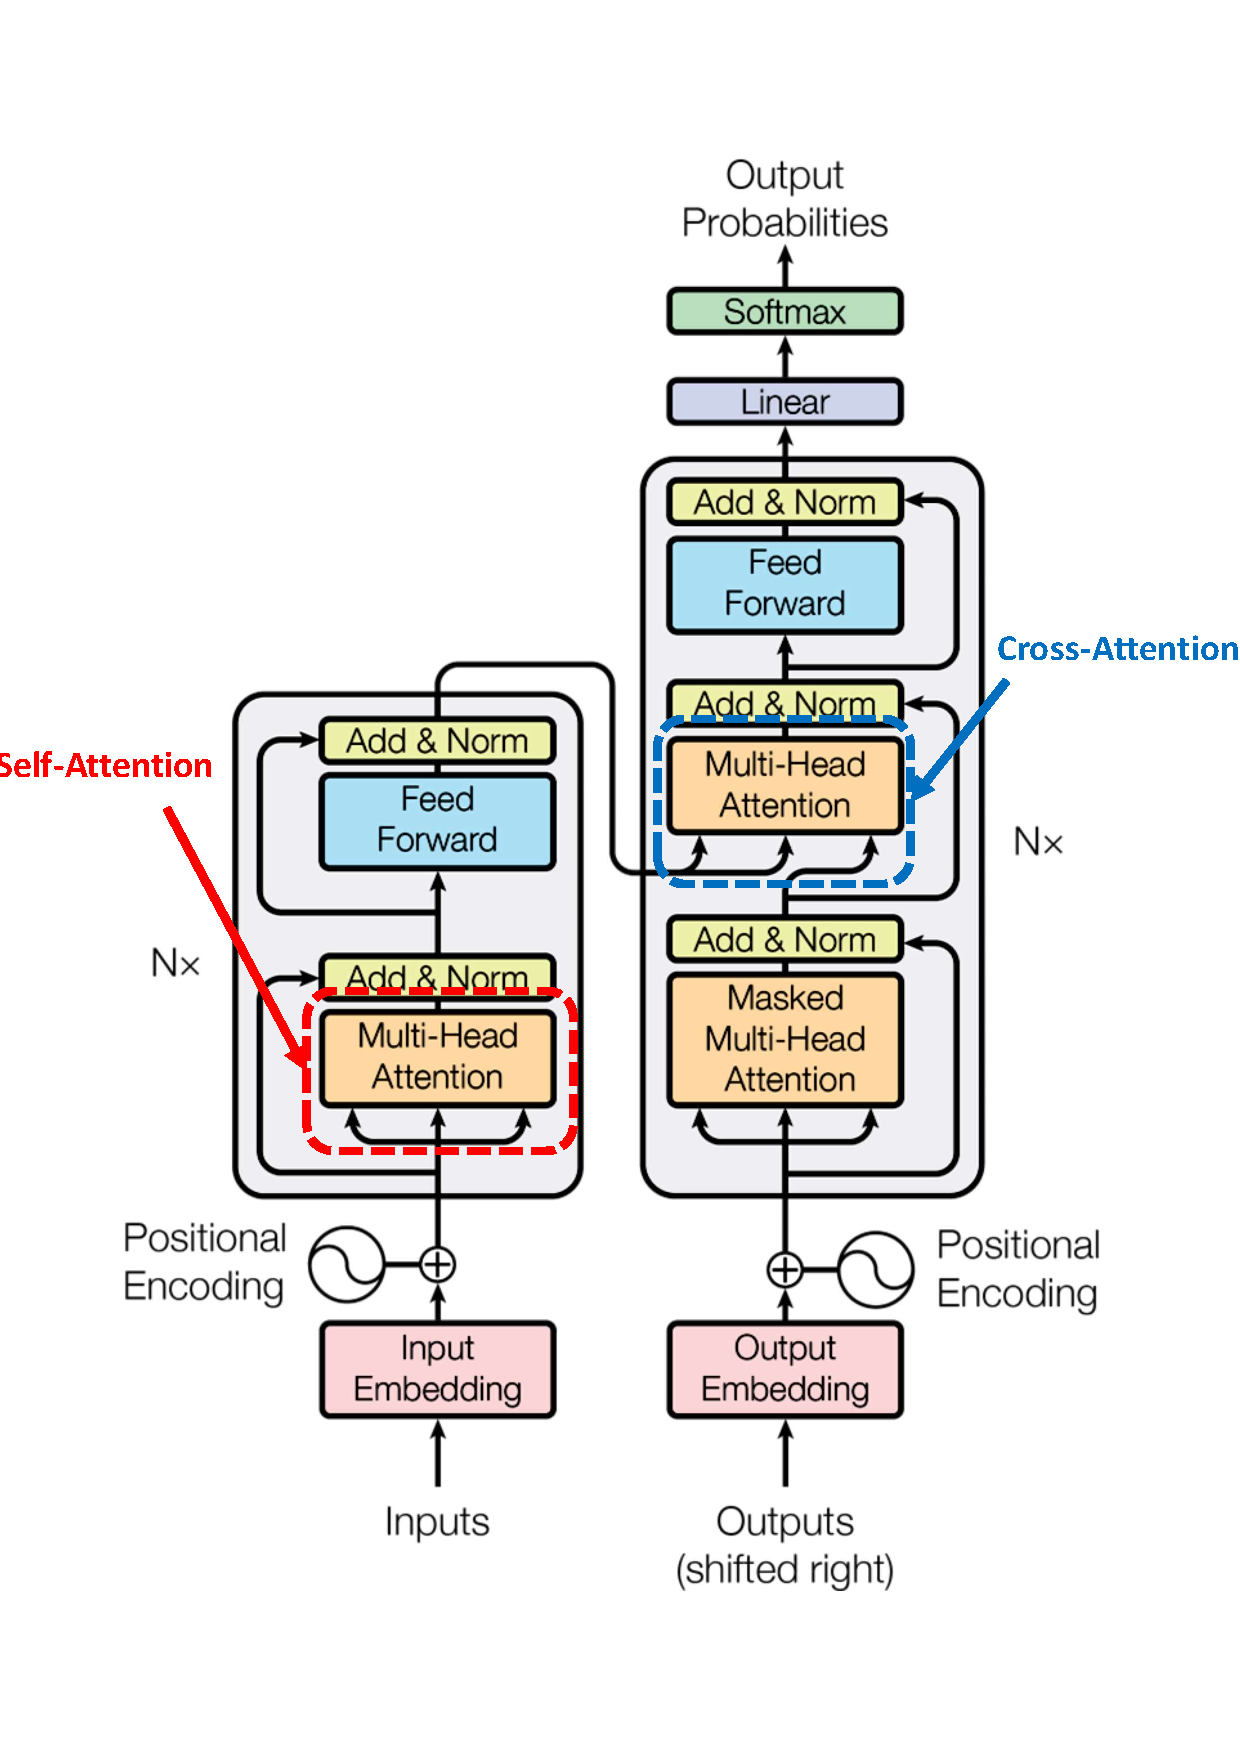
\includegraphics[trim=0cm 2cm 0cm 2cm, width=0.6\linewidth]{chapter_3_theoretical_background/transformer.pdf}
	\caption{Overview of the Transformer architecture}
	Source: \textit{Attention Is All You Need} \cite{vaswani2017attention}
	\label{fig:chapter_3_theoretical_background/transformer}
\end{figure}

The Transformer architecture consists of an encoder and a decoder. The encoder takes as input a sequence of embeddings, such as word embeddings or character embeddings, and produces a sequence of hidden states that capture the information in the input sequence. The decoder takes as input the encoder hidden states and produces a sequence of output embeddings that represent the output sequence.

The encoder consists of multiple layers, each of which contains two sub-layers: a self-attention sub-layer and a feedforward sub-layer. In the self-attention sub-layer, the model computes a representation of each element in the input sequence by attending to all the other elements in the sequence. The feedforward sub-layer applies a pointwise fully connected layer to each position in the sequence independently and identically.

The decoder also consists of multiple layers, each of which contains three sub-layers: a self-attention sub-layer, a cross-attention sub-layer, and a feedforward sub-layer. In the self-attention sub-layer, the model attends to the previously generated output embeddings to compute the next output embedding. In the cross-attention sub-layer, the model attends to the encoder hidden states to incorporate information from the input sequence. The feedforward sub-layer applies a pointwise fully connected layer to each position in the sequence independently and identically.

The Transformer architecture uses residual connections and layer normalization to facilitate training of deep neural networks. Residual connections allow information to flow directly from one layer to another, bypassing the intermediate layers, which can help prevent the vanishing gradient problem. Layer normalization normalizes the input to each sub-layer to have zero mean and unit variance, which can help stabilize the training process. Finally, the original architecture proposes a fully-connected layer and softmax operation to compute the probability distribution over the target vocabulary that determines the words with the highest probability.

Overall, the Transformer architecture has achieved \ac{SOTA} results on a wide range of natural language processing tasks, and its success has led to the development of a variety of transformer-based architectures. As we will see in future sections, Transformers have several advantages over recurrent networks (such as \ac{LSTM}) to encode and decode information with temporal dependencies. Here are some key advantages of transformers:

\begin{itemize}
	\item \textbf{Attention mechanism}: Transformers employ the attention mechanism (both self and cross, if the Transformer decoder is used) that allows them to capture relationships between elements in a sequence more effectively. This mechanism enables the model to focus on relevant elements (or agents, in the field of \ac{MP}) and assign different weights to different words during the encoding and decoding processes. \ac{LSTM} networks, on the other hand, rely on recurrent connections that propagate information sequentially, which may not capture long-range dependencies as effectively as self-attention.
	
	\item \textbf{Parallel Computation}: Transformers are highly parallelizable, meaning that they can process inputs in parallel, which accelerates training and inference. In contrast, \ac{LSTM} networks are inherently sequential in nature, as the recurrent connections require information from previous time steps to be processed before moving on to the next step. This sequential nature limits the parallelizability of \ac{LSTM} networks and can result in slower training and inference times.
	
	\item \textbf{Long-term Dependency}: Transformers are specifically designed to capture long-term dependencies in sequences. The self-attention mechanism allows the model to consider all positions in the input sequence when making predictions, enabling it to capture dependencies over long distances. \ac{LSTM} networks, although capable of capturing short-term dependencies, can struggle with capturing long-term dependencies due to the vanishing or exploding gradient problem.
	
	\item \textbf{Transfer Learning}: Transformers have shown to be highly effective for transfer learning tasks. Pretrained transformer models, such as BERT (Bidirectional Encoder Representations from Transformers), have been trained on large-scale datasets and can be fine-tuned for specific downstream tasks with relatively small amounts of task-specific data. \ac{LSTM} networks typically require more task-specific data to achieve good performance, as they don't benefit from the same level of transfer learning capabilities as transformers.
	
	\item \textbf{Handling Variable-length Inputs}: Transformers can handle variable-length inputs more easily than \ac{LSTM} networks. Since transformers process the entire input sequence in parallel, they do not rely on fixed-length input vectors like \ac{LSTM} networks. This flexibility is particularly advantageous for tasks with variable-length inputs, such as the present work, where a traffic scenario may have an undetermined number of agents around the ego-vehicle.
	
\end{itemize}

While transformers have these advantages, it is important to note that \ac{LSTM} networks are still extensively used by the research community. They have been widely used and well-studied in various applications, especially in tasks where sequential information is critical. The choice between transformers and \ac{LSTM} networks depends on the specific requirements of the task at hand. The attention mechanisms (including self-attention, cross-attention and transformer encoder) will be a key component of this thesis in the proposed learning-based models (Chapters \ref{cha:exploring_gan_for_vehicle_mp}, \ref{cha:efficient_baseline_for_mp_in_ad} and specially \ref{cha:improving_multi_agent}).

\subsection{Graphs}
\label{subsec:3_graphs}

% https://arxiv.org/abs/2204.07697
% http://www.deepnlp.org/blog/latex-code-graph-neural-network
% https://towardsdatascience.com/graph-convolutional-networks-deep-99d7fee5706f
% https://www.datacamp.com/tutorial/comprehensive-introduction-graph-neural-networks-gnns-tutorial

A graph is a type of data structure that contains nodes and edges. A node can be a person, place, or thing, and the edges define the relationship between nodes. The edges can be directed and undirected based on directional dependencies. 

Graphs are excellent in dealing with complex problems with relationships and interactions. They are used in pattern recognition, social networks analysis, recommendation systems, and semantic analysis. Creating graph-based solutions is a whole new field that offers rich insights into complex and interlinked datasets. 

Nevertheless, Graph-based data structures have drawbacks, and researchers must understand them before developing graph-based solutions.

\begin{itemize}
	
	\item \textbf{A graph exists in non-euclidean space}. It does not exist in 2D or 3D space, which makes it harder to interpret the data. To visualize the structure in 2D space, various dimensionality reduction tools must be used.
	
	\item \textbf{Graphs are dynamic}, \ie \ they do not have a fixed form. There can be two visually different graphs, but they might have similar adjacency matrix representations. It makes it difficult for us to analyze data using traditional statistical tools.
	
	\item \textbf{Large size and dimensionality} will increase the graph complexity for human interpretations. The dense structure with multiple nodes and thousands of edges is harder to understand and extract insights. 
	
\end{itemize}

\subsubsection{Graph Neural Networks (GNNs)}
\label{subsubsec:3_gnns}

\acfp{GNN} are a class of neural networks that operate on graphs, which are collections of nodes and edges. A typical graph is represented by a set of node features, represented by a matrix $X \in \mathbb{R}^{N \times D}$, where $N$ is the number of nodes, and $D$ is the number of features associated with each node. Each node is also connected to other nodes via edges, which are represented by an adjacency matrix $A \in {0,1}^{N \times N}$, where $A_{ij} = 1$ if there is an edge between nodes $i$ and $j$, and $0$ otherwise, as observed in Figure \ref{fig:chapter_3_theoretical_background/gnn}.

\begin{figure}[h]
	\centering
	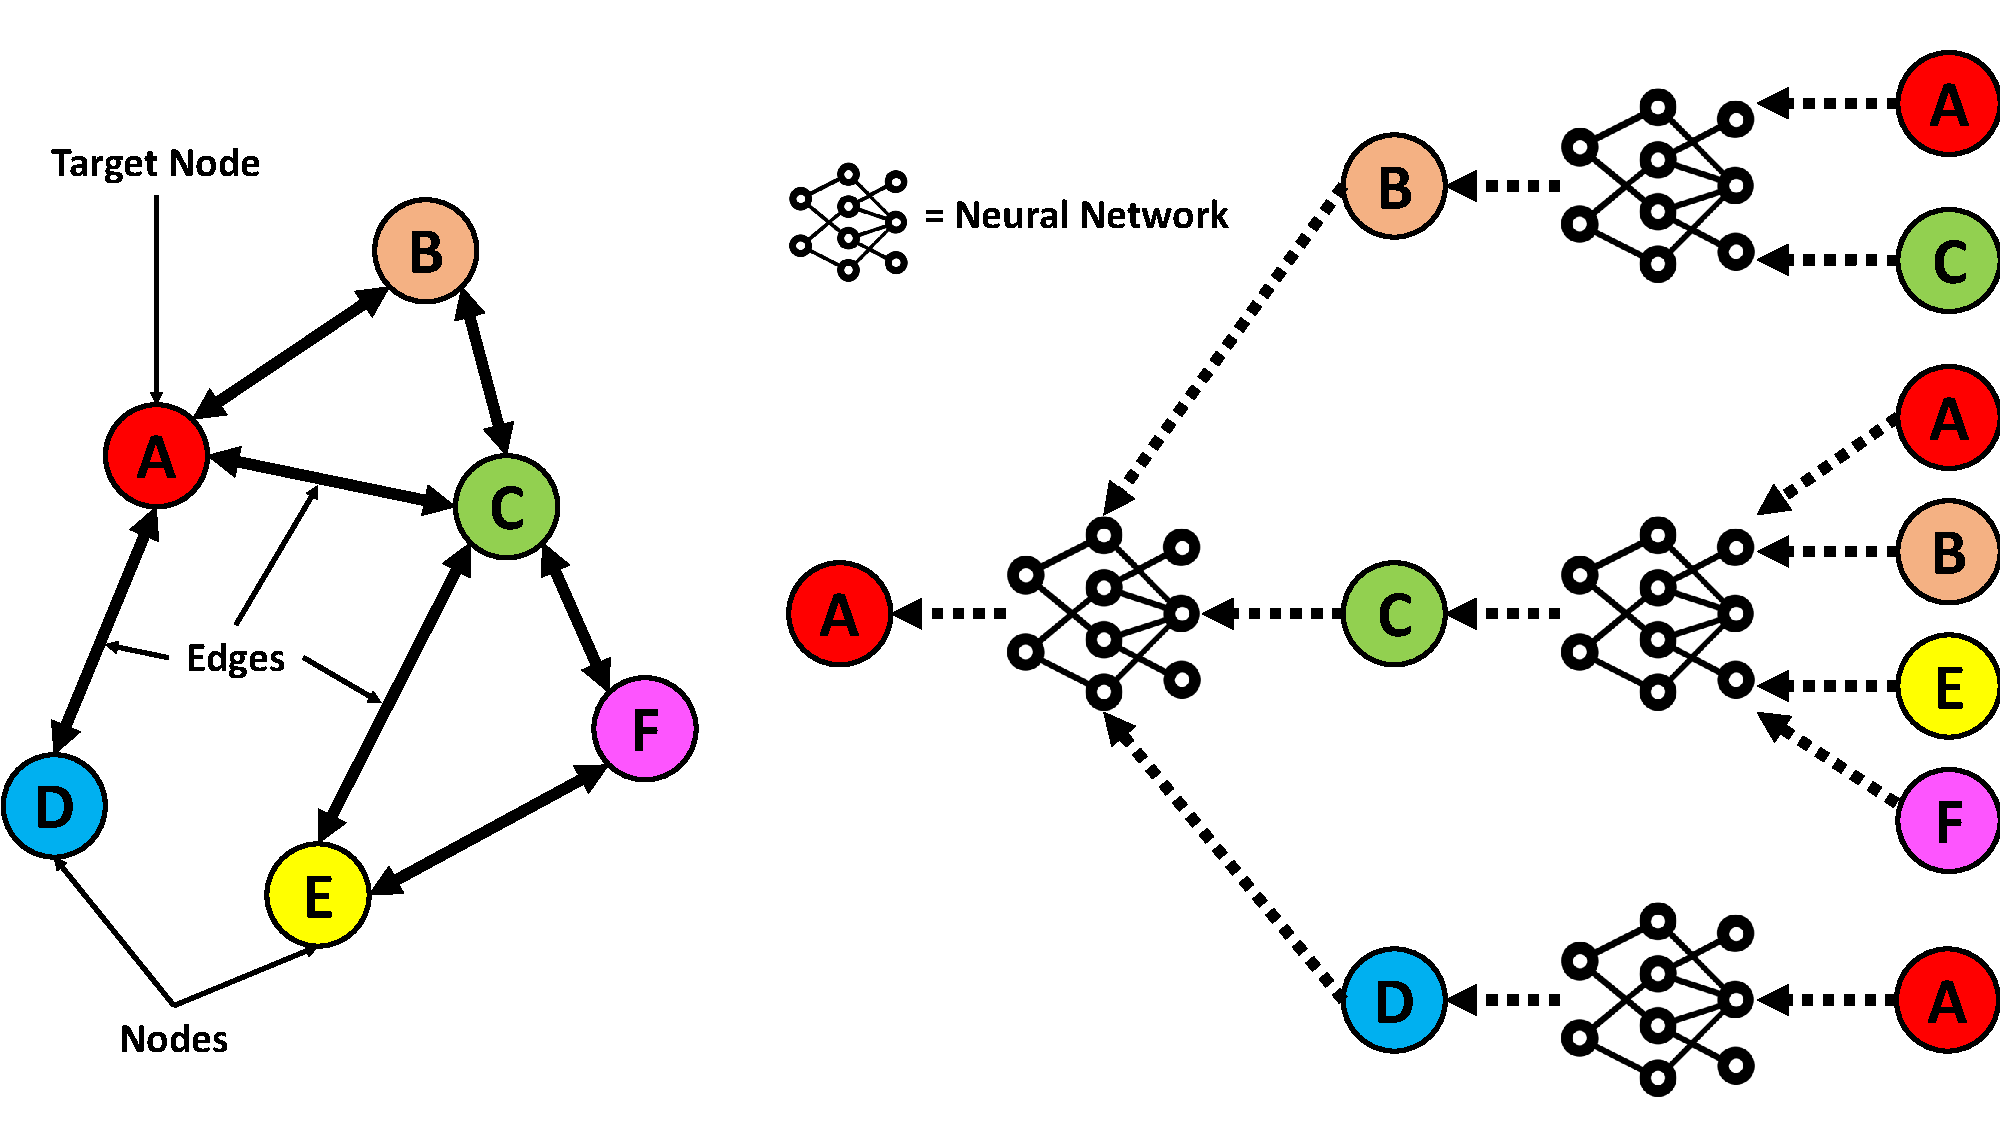
\includegraphics[width=0.8\linewidth]{chapter_3_theoretical_background/input_graph_and_gnn.pdf}
	\captionsetup{justification=justified}
	\caption[Overview of a \ac{GNN}]{Overview of a \ac{GNN}. On the left, it can be observed the input graph of $N$ agents (in this particular case six agents for simplicity) where \textbf{\textcolor{red}{A}} represents the target node over which the influence of neighbouring nodes is going to be calculated. On the right, the latent space of the neighbours is measured as a preliminary stage before aggregating their information to the target node.}
	\label{fig:chapter_3_theoretical_background/gnn}
\end{figure}

The basic idea behind \acp{GNN} is to iteratively update the node representations using information from the graph neighborhood. Specifically, at each iteration, each node aggregates information from its neighbors, and the resulting aggregated representation is used to update the node own representation. This process is typically repeated for multiple iterations until convergence. % GNNs were introduced when Convolutional Neural Networks failed to achieve optimal results due to the arbitrary size of the graph and complex structure. 

One common way to implement this idea is to use the following update rule:

\begin{equation}
h_i^{(l+1)} = f(h_i^{(l)}, \sum_{j} A_{ij} h_j^{(l)})
\end{equation}

where $h_i^{(l)}$ is the representation of node $i$ at iteration $l$, $f$ is a non-linear activation function, and $\sum_{j} A_{ij} h_j^{(l)}$ is the sum of the representations of the neighbours of node $i$ at iteration $l$ (as stated above, $j$ represents the neighbour node).

By stacking multiple layers of such updates, a \ac{GNN} can learn increasingly complex representations of the graph.

There are several types of neural networks, such as:

\begin{itemize}
	
	\item \textbf{Graph Auto-Encoder Networks}, which learn graph representation using an encoder and attempt to reconstruct input graphs using a decoder. They are commonly used in link prediction as Auto-Encoders and are good at dealing with class balance. 
	
	\item \textbf{Recurrent Graph Neural Networks(RGNNs)} are able to learn the best diffusion pattern, and they can handle multi-relational graphs where a single node has multiple relations. They are commonly used in generating text, machine translation, speech recognition or generating image descriptions.
	
	\item \textbf{Gated Graph Neural Networks (GGNNs)} improve Recurrent Graph Neural Networks by adding a node, edge, and time gates on long-term dependencies, being the common uses similar to RGNNs.
	
\end{itemize}

Nevertheless, in this work we focus on a particular type of \ac{GNN}, that is, \acfp{GCN}, which are the most common type of \ac{GNN} used in the field of \ac{MP} for \ac{AD}.

\subsubsection{Graph Convolutional Networks (GCNs)}
\label{subsubsec:3_gcns}

The majority of \acp{GNN} are \acfp{GCN}, which are a specific type of \ac{GNN} that use convolutional operations to aggregate information from the graph neighborhood. \acp{GCN} were introduced when \ac{CNN} failed to achieve optimal results due to the arbitrary size of the graph and complex structure. The basic idea behind \acp{GCN} is to treat the graph as a signal and use convolutional operations to extract features by inspecting neighboring nodes. \acp{GCN} aggregate node vectors, pass the result to the dense layer, and apply non-linearity using the activation function. 

\begin{figure}[h]
	\centering
	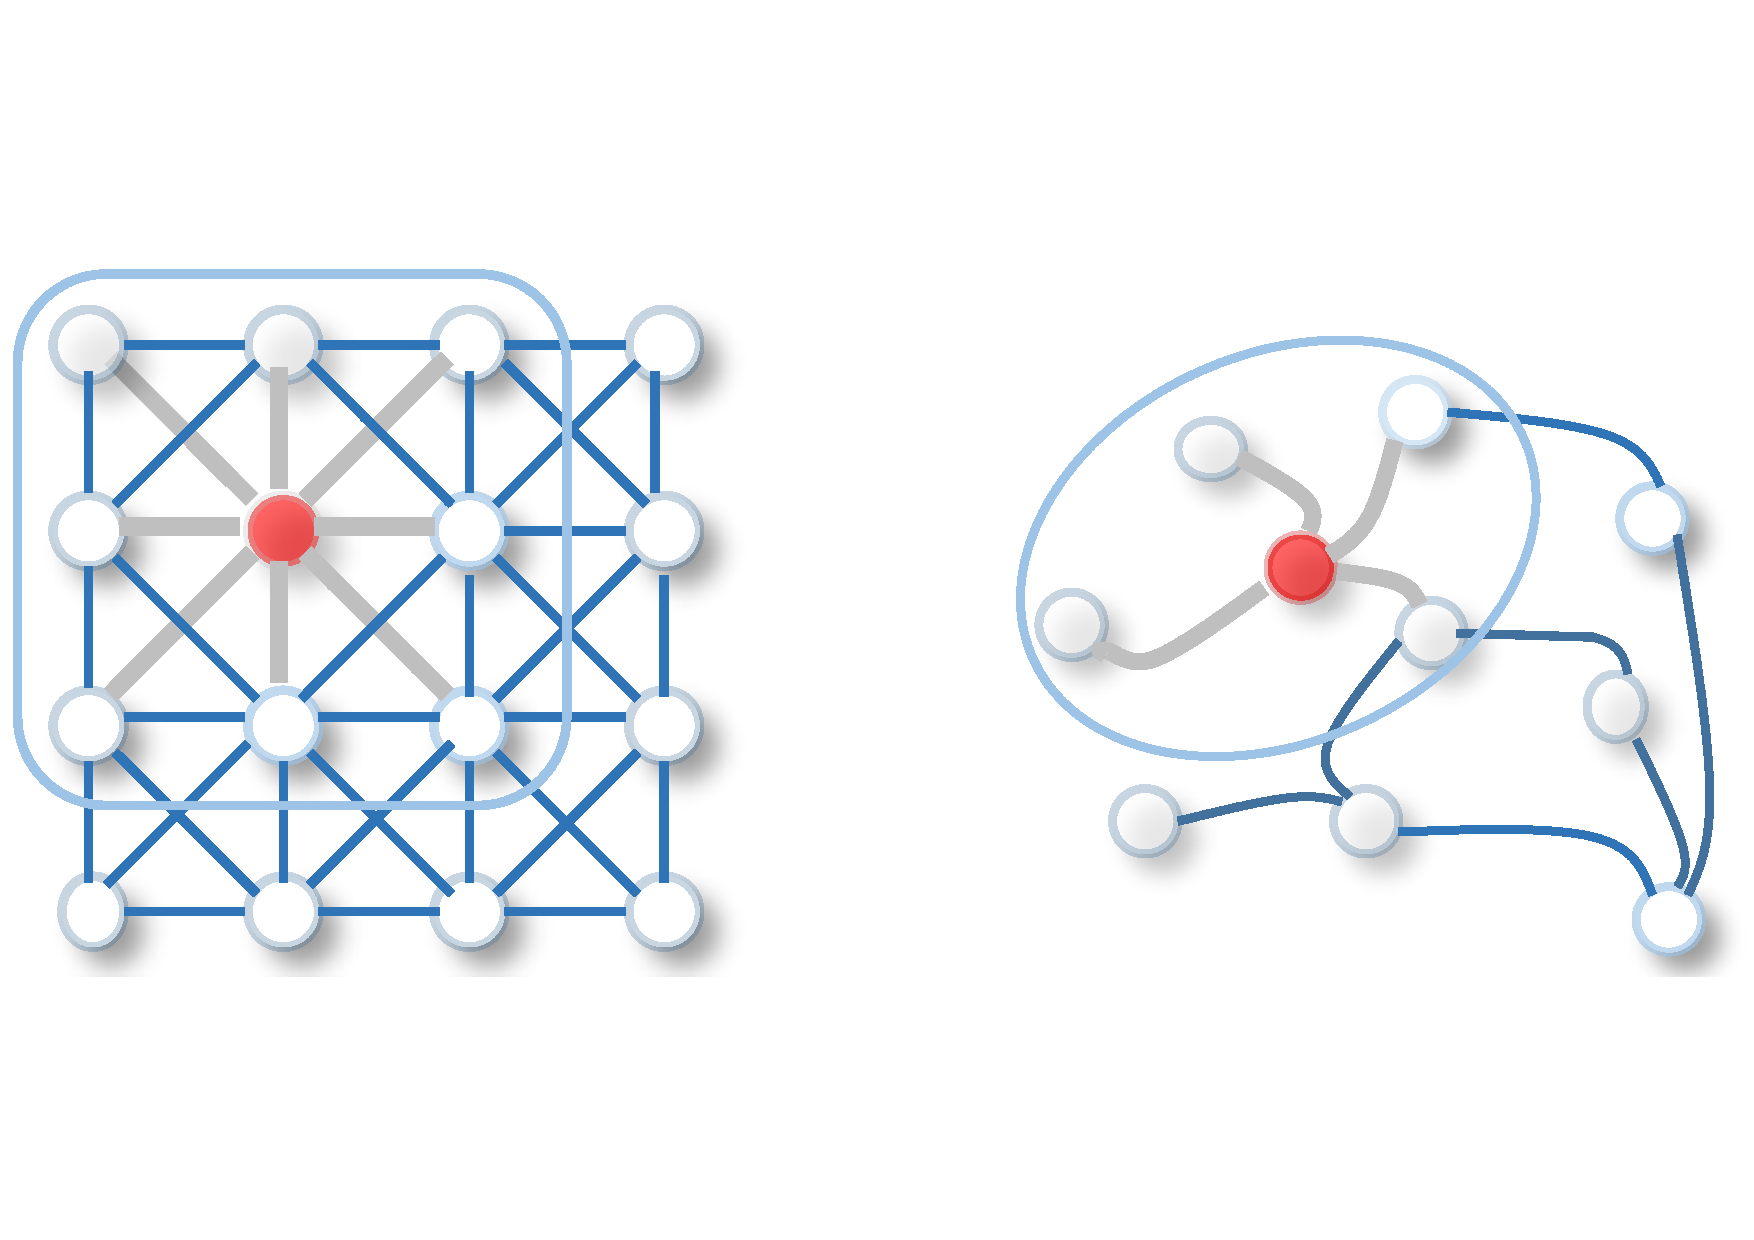
\includegraphics[trim=0cm 3cm 0cm 3cm, width=0.6\linewidth]{chapter_3_theoretical_background/gcn_vs_cnn.pdf}
	\caption[Overview of the sliding kernel of a 2D-CNN vs GCN]{Overview of the sliding kernel of a 2D-CNN vs GCN \\ 
	Source: \textit{A comprehensive survey on graph neural networks} \cite{wu2020comprehensive}}
	\label{fig:chapter_3_theoretical_background/gcn_vs_cnn}
\end{figure}

The major difference between \ac{GCN} and \ac{CNN} is that it is developed to work on non-euclidean data structures where the order of nodes and edges can vary, as it can be appreciated in Figure \ref{fig:chapter_3_theoretical_background/gcn_vs_cnn}. In the 2D convolution operation, each pixel in an image is taken as a node where neighbours are determined by the filter size. The 2D convolution takes the weighted average of pixel values of the red node along with its neighbors. The neighbours of a node are ordered and have a fixed size. On the other hand, to get a hidden representation of a given node red, one simple solution of the graph convolutional operation is to take the average value of the node features of the red node along with its neighbors. Different from image data, the neighbors of a node are unordered and variable in size.

The convolution in \ac{GCN} is the same as a convolution in \acp{CNN}. It multiplies neurons with weights (filters) to learn from data features. A convolutional operation on a graph is defined as:

\begin{equation}
H^{(l+1)} = \sigma(D^{-\frac{1}{2}} A D^{-\frac{1}{2}} H^{(l)} W^{(l)})
\end{equation}

where $H^{(l)}$ is the matrix of node representations at iteration $l$, $W^{(l)}$ is the weight matrix of the $l$-th layer, $A$ is the adjacency matrix of the graph, $D$ is the degree matrix of the graph, and $\sigma$ is a non-linear activation function. Note that in the mathematical field of algebraic graph theory, the degree matrix of an undirected graph is a diagonal matrix which contains information about the degree of each vertex, that is, the number of edges attached to each vertex

The operation $D^{-\frac{1}{2}} A D^{-\frac{1}{2}}$ is a normalization step that scales the adjacency matrix by the inverse square root of the degree matrix. This normalization ensures that nodes with different degrees have similar influence in the convolutional operation. By stacking multiple layers of such convolutions, a \ac{GCN} can learn increasingly complex features of the graph.

\subsection{Training}
\label{subsec:3_training}

Training is the process of iterating through a dataset to make the network learn the optimal mapping (combination of weights) from input to desired output in the data samples. In each iteration, a forward pass through the network is performed, computing the output of each layer until the end. This produces the output response of the network, which is then compared to a desired output through a defined Loss function ($\mathcal{L}$). This function estimates the output error, which is back-propagated through the network to update its weights with the aim of minimizing the error. 

Regarding the supervised training paradigm, backpropagation \cite{rumelhart1995backpropagation} is an algorithm used for training artificial neural networks to update the weights and biases of the neurons in the multi-layer network based on the error between the predicted output and the actual output.

\begin{figure}[h]
	\centering
	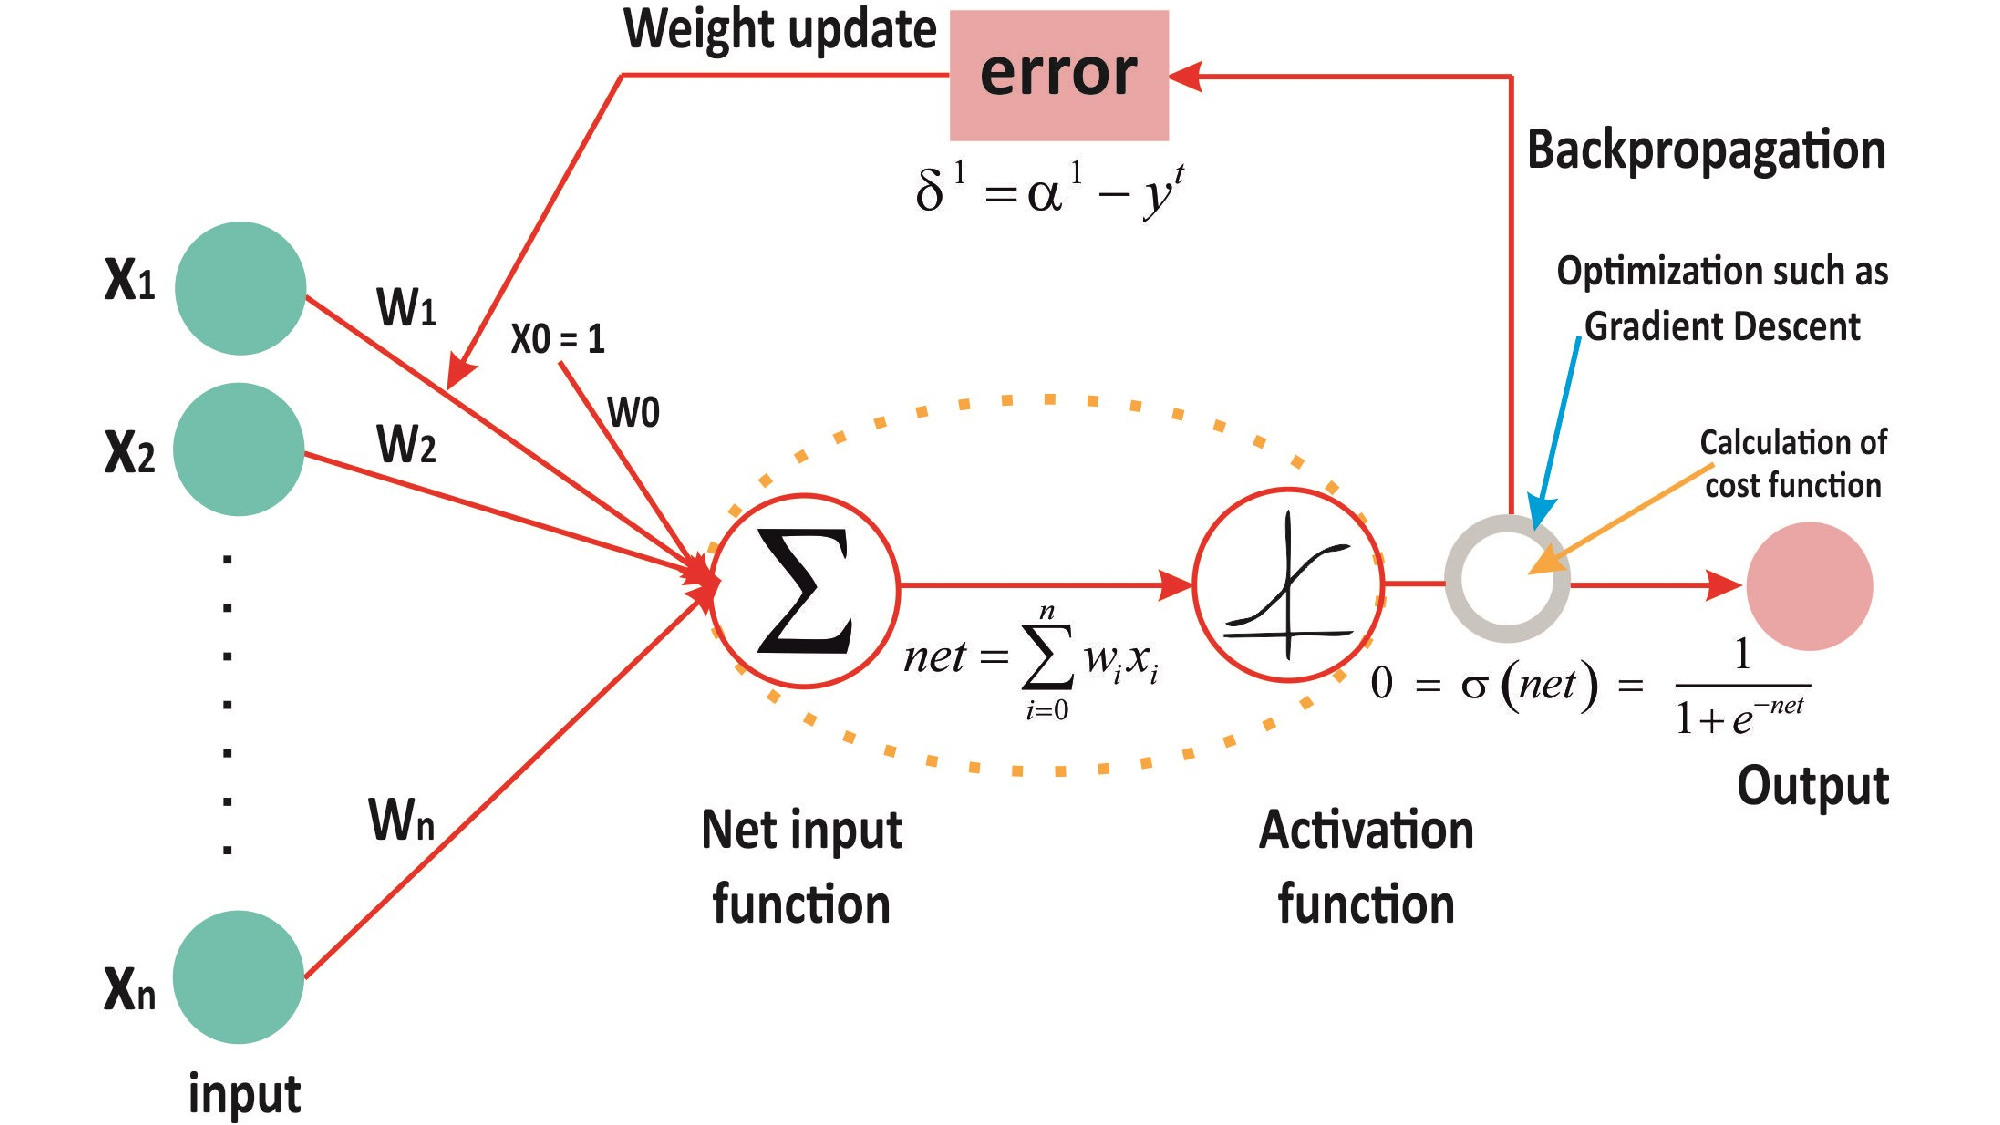
\includegraphics[width=0.8\linewidth]{chapter_3_theoretical_background/backpropagation.pdf}
	\caption[Gradient Descent and Backpropagation]{Gradient Descent and Backpropagation \\ 
	Source: \textit{Backpropagation: The basic theory} \cite{rumelhart1995backpropagation}}
	\label{fig:chapter_3_theoretical_background/backpropagation}
\end{figure}

The backpropagation (Figure \ref{fig:chapter_3_theoretical_background/backpropagation}) algorithm consists of two phases: the forward pass and the backward pass. During the forward pass, the input is fed into the network and propagated through the layers to obtain the predicted output. During the backward pass, the error between the predicted output and the actual output is computed and used to update the weights and biases of the neurons in the network. This algorithm is based on the chain rule of calculus, which allows the gradient of the loss function with respect to each weight and bias to be computed recursively from the output layer to the input layer of the network. The gradient descent algorithm is then used to update the weights and biases in the direction of the negative gradient of the loss function. In that sense, the main losses used in this work are described throughout the remaining content of this Chapter.

\subsubsection{Optimizer and learning rate}
\label{subsubsec:3_optimizer_and_lr}

There are several optimizers commonly used for training deep neural networks in the literature, such as Stochastic Gradient Descent (SGD) \cite{robbins1951stochastic}, Adagrad \cite{duchi2011adaptive}, Root Mean Square Propagation (RMSprop) \cite{zou2019sufficient} or Adadelta \cite{zeiler2012adadelta}. In this work we use one of the most extended, the \ac{ADAM} \cite{kingma2014adam} optimizer. It is a popular optimization algorithm used in deep learning, particularly for training neural networks. It is an adaptive learning rate optimization algorithm that is well suited for large datasets and high-dimensional parameter spaces.

The basic idea behind \ac{ADAM} is to compute adaptive learning rates for each parameter based on estimates of the first and second moments of the gradients. The algorithm computes a moving average of the gradients and their squared values, and uses these estimates to update the parameters with a learning rate that adapts to the local curvature of the loss function. The algorithm also includes bias-correction terms to ensure that the estimates are unbiased, especially in the early stages of training when the estimates are highly uncertain.

The update rule for \ac{ADAM} can be expressed mathematically as follows:

\begin{equation}
\begin{split}
	m_t &= \beta_1 m_{t-1} + (1-\beta_1) g_t \\
	v_t &= \beta_2 v_{t-1} + (1-\beta_2) g_t^2 \\
	\hat{m}_t &= \frac{m_t}{1-\beta_1^t} \\
	\hat{v}t &= \frac{v_t}{1-\beta_2^t} \\
	\theta{t+1} &= \theta_t - \frac{\alpha}{\sqrt{\hat{v}_t}+\epsilon} \hat{m}_t
\end{split}
\end{equation}

where $\theta_t$ is the parameter vector at time step $t$, $g_t$ is the gradient vector, $m_t$ and $v_t$ are the first and second moment estimates at time step $t$, $\hat{m}_t$ and $\hat{v}_t$ are the bias-corrected moment estimates, $\alpha$ is the learning rate, $\beta_1$ and $\beta_2$ are the decay rates for the moment estimates, and $\epsilon$ is a small constant to prevent division by zero.

The algorithm starts with initializing $m_0$ and $v_0$ as zero vectors, and $\theta_0$ as the initial parameter vector. At each iteration, the gradient vector $g_t$ is computed using a batch of training data, and the moment estimates $m_t$ and $v_t$ are updated according to the first two lines of the update rule. The bias-corrected moment estimates $\hat{m}_t$ and $\hat{v}_t$ are then computed using the next two lines of the update rule. Finally, the parameter vector $\theta_t$ is updated using the last line of the update rule.

The hyperparameters $\alpha$, $\beta_1$, $\beta_2$, and $\epsilon$ can be tuned to optimize performance on a particular dataset and neural network architecture.

On the other hand, the learning rate is a key hyperparameter in the optimization process of machine learning algorithms, including optimizer updates like the \ac{ADAM} optimizer. The learning rate controls the step size taken in the direction of the negative gradient during each iteration of the optimization process.

If the learning rate is too small, the optimization process will be slow and may get stuck in local minima. On the other hand, if the learning rate is too large, the optimization process may overshoot the minimum and oscillate back and forth, or even diverge.

In the context of the \ac{ADAM} optimizer, the learning rate is used to adjust the size of the update step taken in the direction of the estimated gradient. The update step is multiplied by the learning rate, which determines the size of the step. A larger learning rate will result in larger update steps, and a smaller learning rate will result in smaller update steps.

In practice, the learning rate is usually set through a process called hyperparameter tuning, where different values of the learning rate are tried on a validation set to find the optimal value that results in the best performance of the model on the test set.

One common technique to adjust the learning rate during training is called learning rate scheduling. This involves decreasing the learning rate over time, often according to a predetermined schedule or based on the performance of the model on a validation set. This technique can help improve the convergence and stability of the optimization process, particularly in the later stages of training when the model is close to the optimal solution.

Overall, the learning rate plays a crucial role in the optimization process of machine learning algorithms, including optimizer updates like the \ac{ADAM} optimizer. Selecting an appropriate learning rate is important for achieving fast and stable convergence to the optimal solution.

In this thesis, we will use the \ac{ADAM} optimizer and learning rate scheduler in Chapters \ref{cha:exploring_gan_for_vehicle_mp}, \ref{cha:efficient_baseline_for_mp_in_ad} and \ref{cha:improving_multi_agent}. Particularly, in terms of the learning rate scheduler, we will make use of the well-established \textit{ReduceLROnPlateau}, which reduces the learning rate when a certain metric of interest (in our case, \ac{minADE}) has stopped improving for a pre-defined \textit{patience} (\ie \ number of epochs over the dataset).

\subsubsection{Losses}
\label{subsubsec:3_losses}

In this Section we explore the different losses that will be employed in order to train the \ac{DL}-based \ac{MP} algorithms in Chapter \ref{cha:exploring_gan_for_vehicle_mp}, \ref{cha:efficient_baseline_for_mp_in_ad} and \ref{cha:improving_multi_agent}.

\paragraph{Regression losses}
\label{par:3_regressions_losses}

% https://blmoistawinde.github.io/ml_equations_latex/

A regression loss is a type of loss function used in regression problems to measure the difference between the predicted and true values of a continuous variable. In other words, it is a way to quantify how well a machine learning model is able to predict numerical values based on input data.

In regression problems, the goal is to learn a function that maps input features to output values. A regression loss is used to train the model by penalizing the difference between the predicted and true output values. The loss function is typically minimized during training, so that the model learns to make more accurate predictions. There are several types of regression loss functions, such as the Quantile loss, Log-Cosh or Mean Absolute Error (MAE). In this work we mainly focus on the \ac{MSE} and SmoothL1 losses, also known as the Huber loss.

\subparagraph{Mean Square Error (MSE) loss}
\label{subpar:3_mse_loss}

The \acf{MSE} loss is a commonly used loss function in regression problems. It measures the average squared difference between the predicted and true values of a continuous variable. The \ac{MSE} loss is given by:

\begin{equation}
	MSE(y, \hat{y}) = \frac{1}{n}\sum_{i=1}^{n}(y_i - \hat{y_i})^2
\end{equation}

where $y_i$ is the true value of the $i$-th data point, $\hat{y_i}$ is the predicted value, and $n$ is the number of data points.

The \ac{MSE} loss penalizes large errors more strongly than small errors, since it uses the square of the difference between the predicted and true values. This makes it sensitive to outliers and can lead to overfitting if the data contains extreme values.

The MSE loss is used in many regression problems, such as linear regression or polynomial regression. It is often used as a performance metric to evaluate the performance of the model predictions.

\subparagraph{SmoothL1 loss}
\label{subpar:3_smoothL1_loss}

The SmoothL1 loss, also known as Huber loss, is a loss function used in regression problems to measure the difference between the predicted and true values of a continuous variable. It is a variant of the L1 loss that is less sensitive to outliers and has a smooth gradient near zero.

The SmoothL1 loss function can be defined as follows:

\begin{equation}
\begin{split}
	L(y, \hat{y}) = \begin{cases}
		\frac{1}{2}(y - \hat{y})^2 & \text{if } |y - \hat{y}| < 1 \\
		|y - \hat{y}| - \frac{1}{2} & \text{otherwise} \
	\end{cases}
\end{split}
\end{equation}

where $y$ is the true value, $\hat{y}$ is the predicted value, $|y - \hat{y}|$ corresponds to the $L_1$ loss (absolute error or distance) and $\frac{1}{2}(y - \hat{y})^2$ corresponds to the $L_2$ loss (Euclidean error or distance).

The SmoothL1 loss function behaves like the L1 loss for small errors and like the $\mathcal{L}_2$ (\aka \ Euclidean distance) loss for large errors. Specifically, for errors smaller than 1, it uses the squared difference between the predicted and true values ($\mathcal{L}_2$), which has a smooth gradient. For larger errors, it uses the absolute difference ($\mathcal{L}_1$), which is less sensitive to outliers than the squared difference.

The SmoothL1 loss is used in regression problems when the data contains outliers or when the model needs to be less sensitive to large errors. It is commonly used in object detection and localization tasks, where the predicted bounding boxes can be highly sensitive to small changes in the input data.

\paragraph{Softmax loss}
\label{par:3_softmax_loss}

The softmax loss, also known as the cross-entropy loss, is a commonly used loss function in classification problems. It measures the difference between the predicted probability distribution and the true probability distribution of a categorical variable. The softmax loss is given by:

\begin{equation}
	CE(y, \hat{y}) = -\frac{1}{n}\sum_{i=1}^{n}\sum_{j=1}^{k} y_{i,j}\log(\hat{y_{i,j}})
\end{equation}

where $y_{i,j}$ is the true probability of the $i$-th data point belonging to class $j$, $\hat{y_{i,j}}$ is the predicted probability, $n$ is the number of data points, and $k$ is the number of classes.

The softmax function is applied to the output of the model to obtain a probability distribution over the classes. The predicted probability of class $j$ is given by:

\begin{equation}
	\hat{y_{i,j}} = \frac{e^{z_{i,j}}}{\sum_{l=1}^{k} e^{z_{i,l}}}
\end{equation}

where $z_{i,j}$ is the unnormalized score or logit for class $j$ of the $i$-th data point.

The softmax loss penalizes the model more heavily for predictions that are far from the true probabilities. It encourages the model to assign higher probabilities to the correct classes and lower probabilities to the incorrect classes.

The softmax loss is used in many classification problems, such as image classification, natural language processing, and speech recognition. It is often used as a performance metric to evaluate the quality of the model predictions.

\paragraph{Negative Log-Likelihood (NLL) loss}
\label{par:3_NLL_loss}

The \acf{NLL} loss is a loss function commonly used in classification problems, particularly in deep learning models that output probabilities for each class. It is a type of Maximum Likelihood Estimation (MLE) loss, which means it attempts to maximize the similarity between the predicted probability distribution and the true probability distribution of the target classes.

The NLL loss function can be defined as follows:

\begin{equation}
	L(y_i, \hat{y_i}) = -\log(\hat{y_{i,y_i}})
\end{equation}

where $y_i$ is the true label of the $i$-th data point, $\hat{y_i}$ is the predicted probability distribution for that point, and $\hat{y_{i,y_i}}$ is the predicted probability for the true label.

This penalizes the model for assigning low probabilities to the true label, while rewarding it for assigning high probabilities. It is a logarithmic loss function, which means that the penalty for low probabilities increases exponentially as the predicted probability approaches zero.

The \ac{NLL} loss is used in classification problems because it provides a gradient that can be used to update the model parameters during training, in order to improve the accuracy of the predicted probabilities. It is commonly used in conjunction with softmax activation function, which ensures that the predicted probabilities sum to one across all classes.

Nevertheless, after revisiting the literature when developing the multi-modal prediction paradigm, we realized that most works employed the \acf{WTA} and max-margin (\aka \ Hinge) losses to maximize the similarity between the future trajectories and the ground-truth. A comparison between employing the \ac{NLL} loss and \ac{WTA}+Hinge will be further detailed in Chapter \ref{cha:efficient_baseline_for_mp_in_ad}.

\paragraph{Winner-Takes-All loss}
\label{par:3_WTA_loss}

\acf{WTA} loss is a loss function used in clustering problems, particularly in competitive learning models. It is a type of unsupervised learning, which means that it does not require labeled data for training.

The \ac{WTA} loss function can be defined as follows:

\begin{equation}
\begin{split}
	L(y_i, f(x_i)) = \begin{cases}
		0 & \text{if } y_i = \arg\max_j f_j(x_i) \\
		1 & \text{otherwise} \
	\end{cases}
\end{split}
\end{equation}

where $y_i$ is the true cluster of the $i$-th data point, $f_j(x_i)$ is the activation of the $j$-th neuron in the output layer for that point, and $\arg\max_j f_j(x_i)$ is the index of the neuron with the highest activation.

This loss function penalizes the model for assigning a data point to the wrong cluster. It works by forcing each neuron in the output layer to specialize in a particular cluster, such that the neuron with the highest activation for a given point corresponds to the true cluster of that point.

The \ac{WTA} loss is used in clustering problems because it encourages the model to learn a set of representative clusters that capture the structure of the data, without requiring any prior knowledge of the true labels. It is commonly used in conjunction with competitive learning algorithms, such as self-organizing maps (SOMs), that use local competition between neurons to learn a topology-preserving mapping from the input space to the output space.

\paragraph{Hinge loss}
\label{par:3_hinge_loss}

Hinge loss is a loss function used in classification problems, particularly in Support Vector Machines (SVMs). It is a type of max-margin loss, which means it attempts to maximize the margin between the decision boundary and the data points.

The hinge loss function can be defined as follows:

\begin{equation}
	L(y_i, f(x_i)) = \max(0, 1 - y_i f(x_i))
\end{equation}

where $y_i$ is the true label of the $i$-th data point, $f(x_i)$ is the predicted score for that point, and $1$ is a margin hyperparameter that determines the width of the margin.

If $y_i f(x_i) \geq 1$, then the point is correctly classified and the loss is zero. If $y_i f(x_i) < 1$, then the point is misclassified and the loss is proportional to the distance between the predicted score and the correct score. The loss function penalizes misclassifications linearly, with a slope of -1 for negative misclassifications and 0 for positive misclassifications.

The hinge loss is used in SVMs because it encourages the model to find a decision boundary that maximizes the margin between the classes, while still correctly classifying the data points. This results in a more robust and generalizable model.

\subsubsection{Regularization techniques}
\label{subsubsec:3_regularization}

Regularization techniques in deep learning are used to prevent overfitting and improve the generalization performance of a model. Overfitting occurs when a model fits the training data too closely and captures noise or irrelevant patterns, resulting in poor performance on new, unseen data. Here are some commonly used regularization techniques in deep learning, which can be combined and tuned to improve the performance of a model on a specific task or dataset:

\begin{itemize}
	
	\item \textbf{$\mathcal{L}_1$ and $\mathcal{L}_2$} regularization are two popular regularization techniques that add a penalty term to the loss function during training. L1 regularization adds the sum of the absolute values of the weights to the loss function, while $\mathcal{L}_2$ regularization adds the sum of the squares of the weights. This encourages the model to learn simpler and more generalizable representations by shrinking the weights towards zero.
	
	\item \textbf{Dropout} is a regularization technique that randomly drops out some units (neurons) in a layer during training. This forces the remaining units to learn more robust and diverse representations that generalize better to new data. Dropout has been shown to be effective in reducing overfitting, particularly in deep neural networks with many layers.
	
	\item \textbf{Data augmentation} is a technique that artificially increases the size of the training set by generating new examples from existing ones. This can be done by applying transformations such as rotations, translations, flips, or adding noise to the input data. Data augmentation can help reduce overfitting by increasing the diversity of the training data and improving the generalization performance of the model.
	
	\item \textbf{Early stopping} is a technique that monitors the performance of the model on a validation set during training and stops the training process when the performance starts to degrade. This prevents the model from overfitting to the training data and allows it to generalize better to new data.
	
	\item \textbf{Batch normalization} is a technique that normalizes the activations of a layer by subtracting the batch mean and dividing by the batch standard deviation. This helps stabilize the distribution of the activations and reduces the internal covariate shift, which can improve the training process and reduce overfitting.
	
	\item \textbf{Weight decay} is a technique that adds a penalty term to the loss function during training, similar to $\mathcal{L}_2$ regularization. The penalty term is proportional to the square of the weights, and it encourages the model to learn smaller and simpler weights, which can reduce overfitting.
	
\end{itemize}

Moreover, another interesting technique to help the model improve during training is hard-mining. Hard-mining is a technique in \ac{DL} used to improve the training of a model by focusing on the samples that are most difficult to classify correctly. In terms of vehicle \ac{MP}, hard-mining is used to improve the accuracy of predictions by focusing on challenging or critical scenarios. It involves selecting and prioritizing difficult or informative examples during the training process to emphasize learning in those areas. It typically involves identifying and emphasizing challenging situations where accurate prediction is crucial. These situations could include complex traffic interactions, sudden maneuvers, or high-risk scenarios. By focusing on these challenging instances, the model can learn to handle them more effectively and improve its overall prediction capabilities.

Assuming a dataset with a wide range of situations is provided (\eg \ Argoverse 1 and 2 datasets), the process of hard-mining involves several steps:

\begin{enumerate}
	
	\item \textbf{Training}: The model is trained on the annotated dataset using machine learning techniques. During the training process, the model learns to predict future vehicle motions based on the available input data.
	
	\item \textbf{Evaluation and Selection}: After training, we identify in the training dataset the instances where the model performance is suboptimal or where it fails to accurately predict certain behaviors (for example, challenging intersections, sudden accelerations or emergency breaks). These scenarios might include instances where the model fails to predict dangerous maneuvers accurately or struggles with complex interactions.
	
	\item \textbf{Sample Selection}: The challenging examples identified in the previous step are selected as hard-mining samples. These samples are then given more weight or importance during subsequent training iterations.
	
	\item \textbf{Iterative Training}: The model is retrained using the original dataset, giving more emphasis to the hard-mining samples in the batch (\eg \ at least 20 \% of the samples of the batch must be a random subset of total hard-mining samples). By increasing the exposure to challenging scenarios, the model learns to improve its predictions specifically for those cases.
	
	\item \textbf{Iterative Evaluation}: The model performance is evaluated on the validation set, and the hard-mining process is repeated if necessary. This iterative approach allows the model to gradually refine its predictions and adapt to challenging situations more effectively.
	
\end{enumerate}

As observed, by incorporating hard-mining into the training process, vehicle \ac{MP} models can focus on challenging scenarios and improve their generalization and performance in unknown scenarios and critical situations respectively.

\section{Summary}
\label{sec:3_summary}

In this Chapter, the mathematical background of various physics-based and \ac{DL}-based techniques used for \ac{MP} models is thoroughly examined. The Chapter aims to provide a comprehensive understanding of these methods and their applications in the field of motion prediction.

The Chapter begins by introducing the physics-based techniques, starting with the \ac{KF}. The Kalman Filter is a recursive algorithm used to estimate the state of a dynamic system by incorporating noisy measurements. Its mathematical foundation, including the state-space model and the prediction and update steps, is discussed in detail. Next, the \ac{HA} is presented, which is a combinatorial optimization algorithm used for data association in multiple object tracking. The Chapter delves into the mathematical formulation of the Hungarian Algorithm and how it can be applied to motion prediction tasks.

Moving on to the physics-based models, the Chapter explores the \ac{CTRV} and \ac{CTRA} models. These models are widely used for trajectory prediction and capture the motion dynamics of objects by considering their position, velocity, and acceleration. The mathematical equations for these models are examined, highlighting how they can be utilized to predict future motion paths.

The Chapter then transitions to \ac{DL}-based techniques, which have gained significant attention in recent years due to their ability to capture complex patterns and dependencies in data. Several models are discussed in detail, starting with the 1D-\ac{CNN}. The mathematical architecture of the 1D-\ac{CNN} is explained, emphasizing its ability to extract spatial and temporal features from sequential data for motion prediction.

Next, the \ac{LSTM} model is introduced, which is a type of \ac{RNN} specifically designed to handle sequence data. The chapter provides an overview of the \ac{LSTM} architecture, including its memory cell and gate mechanisms, which enable it to capture long-term dependencies and predict future motion accurately.

The chapter then explores \acp{GAN} and their application in motion prediction. \acp{GAN} consist of a generator and discriminator network that compete against each other, resulting in the generation of realistic and coherent motion trajectories. The mathematical formulation of \acp{GAN} and their training process are examined in detail.

Furthermore, the Attention mechanism is examined, which is a component commonly integrated into deep learning models to focus on relevant parts of the input data. The chapter explores the mathematical formulation of the Attention mechanism and its application in motion prediction models, highlighting its ability to assign different weights to different input features based on their relevance.

Then, the \ac{GCN} is discussed, which is a deep learning model capable of operating on graph-structured data. The chapter explains how \acp{GCN} can be used to represent and predict motion patterns in scenarios where objects interact with each other.

Finally, an overview of the training process, including the optimization and backpropagation strategy, the losses covered in this thesis and regularization techniques, are explored. % Overall, this chapter provides a comprehensive overview of the mathematical foundations of the mechanisms and techniques used along this work.